%  A simple AAU report template.
%  2015-05-08 v. 1.2.0
%  Copyright 2010-2015 by Jesper Kjær Nielsen <jkn@es.aau.dk>
%
%  This is free software: you can redistribute it and/or modify
%  it under the terms of the GNU General Public License as published by
%  the Free Software Foundation, either version 3 of the License, or
%  (at your option) any later version.
%
%  This is distributed in the hope that it will be useful,
%  but WITHOUT ANY WARRANTY; without even the implied warranty of
%  MERCHANTABILITY or FITNESS FOR A PARTICULAR PURPOSE.  See the
%  GNU General Public License for more details.
%
%  You can find the GNU General Public License at <http://www.gnu.org/licenses/>.
%
%  A simple AAU report template.
%  2015-05-08 v. 1.2.0
%  Copyright 2010-2015 by Jesper Kjær Nielsen <jkn@es.aau.dk>
%
%  This is free software: you can redistribute it and/or modify
%  it under the terms of the GNU General Public License as published by
%  the Free Software Foundation, either version 3 of the License, or
%  (at your option) any later version.
%
%  This is distributed in the hope that it will be useful,
%  but WITHOUT ANY WARRANTY; without even the implied warranty of
%  MERCHANTABILITY or FITNESS FOR A PARTICULAR PURPOSE.  See the
%  GNU General Public License for more details.
%
%  You can find the GNU General Public License at <http://www.gnu.org/licenses/>.
%
\documentclass[11pt,oneside,a4paper,openright]{report}
%%%%%%%%%%%%%%%%%%%%%%%%%%%%%%%%%%%%%%%%%%%%%%%%
% Language, Encoding and Fonts
% http://en.wikibooks.org/wiki/LaTeX/Internationalization
%%%%%%%%%%%%%%%%%%%%%%%%%%%%%%%%%%%%%%%%%%%%%%%%
% Select encoding of your inputs. Depends on
% your operating system and its default input
% encoding. Typically, you should use
%   Linux  : utf8 (most modern Linux distributions)
%            latin1 
%   Windows: ansinew
%            latin1 (works in most cases)
%   Mac    : applemac
% Notice that you can manually change the input
% encoding of your files by selecting "save as"
% an select the desired input encoding. 
\usepackage[utf8]{inputenc}
% Make latex understand and use the typographic
% rules of the language used in the document.
\usepackage[danish,english,spanish]{babel}
% Use the palatino font
\usepackage[sc]{mathpazo}
\linespread{1.05}         % Palatino needs more leading (space between lines)
% Choose the font encoding
\usepackage[T1]{fontenc}
%%%%%%%%%%%%%%%%%%%%%%%%%%%%%%%%%%%%%%%%%%%%%%%%
% Graphics and Tables
% http://en.wikibooks.org/wiki/LaTeX/Importing_Graphics
% http://en.wikibooks.org/wiki/LaTeX/Tables
% http://en.wikibooks.org/wiki/LaTeX/Colors
%%%%%%%%%%%%%%%%%%%%%%%%%%%%%%%%%%%%%%%%%%%%%%%%
% load a colour package
\usepackage{xcolor}
\definecolor{aaublue}{RGB}{33,26,82}% dark blue
% The standard graphics inclusion package
\usepackage{graphicx}
\usepackage{float} 
% Set up how figure and table captions are displayed
\usepackage{caption}
\usepackage{subcaption}
\captionsetup{%
  font=footnotesize,% set font size to footnotesize
  labelfont=bf % bold label (e.g., Figure 3.2) font
}
% Make the standard latex tables look so much better
\usepackage{array,booktabs}
% Enable the use of frames around, e.g., theorems
% The framed package is used in the example environment
\usepackage{framed}
%Package for showing Youtube videos
\usepackage{media9}
\usepackage{multicol}

%%%%%%%%%%%%%%%%%%%%%%%%%%%%%%%%%%%%%%%%%%%%%%%%
% Mathematics
% http://en.wikibooks.org/wiki/LaTeX/Mathematics
%%%%%%%%%%%%%%%%%%%%%%%%%%%%%%%%%%%%%%%%%%%%%%%%
% Defines new environments such as equation,
% align and split 
\usepackage{amsmath}
% Adds new math symbols
\usepackage{amssymb}
% Use theorems in your document
% The ntheorem package is also used for the example environment
% When using thmmarks, amsmath must be an option as well. Otherwise \eqref doesn't work anymore.
\usepackage[framed,amsmath,thmmarks]{ntheorem}

%%%%%%%%%%%%%%%%%%%%%%%%%%%%%%%%%%%%%%%%%%%%%%%%
% Page Layout
% http://en.wikibooks.org/wiki/LaTeX/Page_Layout
%%%%%%%%%%%%%%%%%%%%%%%%%%%%%%%%%%%%%%%%%%%%%%%%
% Change margins, papersize, etc of the document
\usepackage[
  inner=28mm,% left margin on an odd page
  outer=41mm,
  top = 1cm% right margin on an odd page
  ]{geometry}
% Modify how \chapter, \section, etc. look
% The titlesec package is very configureable
\usepackage{substr}
\usepackage{titlesec}
\titleformat{\chapter}[display]{\normalfont\huge\bfseries}{\chaptertitlename\ \thechapter}{20pt}{\huge}

\titleformat*{\section}{\normalfont\Large\bfseries}
\titleformat*{\subsection}{\normalfont\large\bfseries}
\titleformat*{\subsubsection}{\normalfont\normalsize\bfseries}
%\titleformat*{\paragraph}{\normalfont\normalsize\bfseries}
%\titleformat*{\subparagraph}{\normalfont\normalsize\bfseries}
\usepackage{tocloft}
\renewcommand\cftaftertoctitle{\par\noindent\hrulefill\par\vskip-4.3em}
\renewcommand\cftchapdotsep{\cftdotsep}
% Clear empty pages between chapters
\let\origdoublepage\cleardoublepage
\newcommand{\clearemptydoublepage}{%
  \clearpage
  {\pagestyle{empty}\origdoublepage}%
}
\let\cleardoublepage\clearemptydoublepage

% Change the headers and footers
\usepackage{fancyhdr}
\pagestyle{fancy}
\fancyhf{} %delete everything
\renewcommand{\headrulewidth}{0pt} %remove the horizontal line in the header
\fancyhead[R]{\small\nouppercase Práctica 3. VLSI} %even page - chapter title
\fancyhead[L]{\small\nouppercase\leftmark} %uneven page - section title
\fancyfoot[C]{\thepage}
\raggedbottom
% Enable arithmetics with length. Useful when
% typesetting the layout.
\usepackage{calc}

%%%%%%%%%%%%%%%%%%%%%%%%%%%%%%%%%%%%%%%%%%%%%%%%
% Bibliography
% http://en.wikibooks.org/wiki/LaTeX/Bibliography_Management
%%%%%%%%%%%%%%%%%%%%%%%%%%%%%%%%%%%%%%%%%%%%%%%%
\usepackage[backend=bibtex,
  bibencoding=utf8
  ]{biblatex}
\addbibresource{bib/mybib}
\usepackage{csquotes}
%%%%%%%%%%%%%%%%%%%%%%%%%%%%%%%%%%%%%%%%%%%%%%%%
% Misc
%%%%%%%%%%%%%%%%%%%%%%%%%%%%%%%%%%%%%%%%%%%%%%%%
% Add bibliography and index to the table of
% contents
\usepackage[nottoc]{tocbibind}
% Add the command \pageref{LastPage} which refers to the
% page number of the last page
\usepackage{lastpage}
% Add todo notes in the margin of the document
\usepackage[
%  disable, %turn off todonotes
  colorinlistoftodos, %enable a coloured square in the list of todos
  textwidth=\marginparwidth, %set the width of the todonotes
  textsize=scriptsize, %size of the text in the todonotes
  ]{todonotes}
  
  \usepackage{etaremune}
  \usepackage{changepage}
\usepackage{multicol}
%%%%%%%%%%%%%%%%%%%%%%%%%%%%%%%%%%%%%%%%%%%%%%%%
% Hyperlinks
% http://en.wikibooks.org/wiki/LaTeX/Hyperlinks
%%%%%%%%%%%%%%%%%%%%%%%%%%%%%%%%%%%%%%%%%%%%%%%%
% Enable hyperlinks and insert info into the pdf
% file. Hypperref should be loaded as one of the 
% last packages
\usepackage{hyperref}
\hypersetup{%
	plainpages=false,%
	pdfauthor={Author(s)},%
	pdftitle={Title},%
	pdfsubject={Subject},%
	bookmarksnumbered=true,%
	colorlinks=false,%
	citecolor=black,%
	filecolor=black,%
	linkcolor=black,% you should probably change this to black before printing
	urlcolor=black,%
	pdfstartview=FitH%
}
%%%%%%%%%%%%%%%%%%%%%%%%%%%%%%%%%%%%%%%%%%%%%%%%
% Java Language
%https://tex.stackexchange.com/questions/377122/typesetting-for-a-verilog-lstinput%
%%%%%%%%%%%%%%%%%%%%%%%%%%%%%%%%%%%%%%%%%%%%%%%%

\definecolor{pblue}{rgb}{0.13,0.13,1}
\definecolor{pgreen}{rgb}{0,0.5,0}
\definecolor{pred}{rgb}{0.9,0,0}
\definecolor{pgrey}{rgb}{0.46,0.45,0.48}
\usepackage{inconsolata}
\usepackage{listings}
\usepackage{tcolorbox}
\lstset{language=Java,
  showspaces=false,
  showtabs=false,
  breaklines=true,
  showstringspaces=false,
  breakatwhitespace=true,
  commentstyle=\color{pgreen},
  keywordstyle=\color{pblue},
  stringstyle=\color{pred},
  basicstyle=\ttfamily,
  morecomment=[s][\color{gray}]{@}{\ }
  moredelim=[is][\textcolor{pgrey}]{\%\%}{\%\%}
}
\tcbuselibrary{listings,skins}
\lstdefinestyle{mystyle}{
numbers=left, 
numberstyle=\small, 
numbersep=8pt, 
language=Java
}

\newtcblisting{mylisting}[2][]{
    arc=0pt, outer arc=0pt,
    listing only,
    listing style=mystyle,
    title=#2,
    #1
    }
    
\usepackage{trace}
\usepackage{dirtytalk}% package inclusion and set up of the document
% see, e.g., http://en.wikibooks.org/wiki/LaTeX/Formatting#Hyphenation
% for more information on word hyphenation
\hyphenation{ex-am-ple hy-phen-a-tion short}
\hyphenation{long la-tex}% 
%  A simple AAU report template.
%  2015-05-08 v. 1.2.0
%  Copyright 2010-2015 by Jesper Kjær Nielsen <jkn@es.aau.dk>
%
%  This is free software: you can redistribute it and/or modify
%  it under the terms of the GNU General Public License as published by
%  the Free Software Foundation, either version 3 of the License, or
%  (at your option) any later version.
%
%  This is distributed in the hope that it will be useful,
%  but WITHOUT ANY WARRANTY; without even the implied warranty of
%  MERCHANTABILITY or FITNESS FOR A PARTICULAR PURPOSE.  See the
%  GNU General Public License for more details.
%
%  You can find the GNU General Public License at <http://www.gnu.org/licenses/>.
%
%
%
% see, e.g., http://en.wikibooks.org/wiki/LaTeX/Customizing_LaTeX#New_commands
% for more information on how to create macros

%%%%%%%%%%%%%%%%%%%%%%%%%%%%%%%%%%%%%%%%%%%%%%%%
% Macros for the titlepage
%%%%%%%%%%%%%%%%%%%%%%%%%%%%%%%%%%%%%%%%%%%%%%%%
%Creates the aau titlepage
\newcommand{\aautitlepage}[3]{%
  {
    %set up various length
    \ifx\titlepageleftcolumnwidth\undefined
      \newlength{\titlepageleftcolumnwidth}
      \newlength{\titlepagerightcolumnwidth}
    \fi
    \setlength{\titlepageleftcolumnwidth}{0.5\textwidth-\tabcolsep}
    \setlength{\titlepagerightcolumnwidth}{\textwidth-2\tabcolsep-\titlepageleftcolumnwidth}
    %create title page
    \thispagestyle{empty}
    \noindent%
    \begin{tabular}{@{}ll@{}}
      \parbox{\titlepageleftcolumnwidth}{
        \iflanguage{danish}{%
          \includegraphics[width=\titlepageleftcolumnwidth]{figures/aau_logo_da}
        }{%
          
\includegraphics[width=\titlepageleftcolumnwidth]{figures/UPV_logo.pdf}
        }
      } &
      \parbox{\titlepagerightcolumnwidth}{\raggedleft\sf\small
        #2
      }\bigskip\\
       #1 &
      \parbox[t]{\titlepagerightcolumnwidth}{%
      \textbf{Abstract:}\bigskip\par
        \fbox{\parbox{\titlepagerightcolumnwidth-2\fboxsep-2\fboxrule}{%
          #3
        }}
      }\\
    \end{tabular}
    \vfill
    \iflanguage{danish}{%
      \noindent{\footnotesize\emph{Rapportens indhold er frit tilgængeligt, men offentliggørelse (med kildeangivelse) må kun ske efter aftale med forfatterne.}}
    }{%
      
    }
    \clearpage
  }
}

%Create english project info
\newcommand{\englishprojectinfo}[8]{%
  \parbox[t]{\titlepageleftcolumnwidth}{
    \textbf{Título:}\\ #1\bigskip\par
    \textbf{Tema:}\\ #2\bigskip\par
    \textbf{Periodo:}\\ #3\bigskip\par
    \textbf{Grupo:}\\ #4\bigskip\par
    \textbf{Participantes:}\\ #5\bigskip\par
    \textbf{Profesores:}\\ #6\bigskip\par
    \textbf{Copias:} #7\bigskip\par
    \textbf{Número de páginas:} \pageref{LastPage}\bigskip\par
    \textbf{Fecha de finalización:}\\ #8
  }
}

%Create danish project info
\newcommand{\danishprojectinfo}[8]{%
  \parbox[t]{\titlepageleftcolumnwidth}{
    \textbf{Titel:}\\ #1\bigskip\par
    \textbf{Tema:}\\ #2\bigskip\par
    \textbf{Projektperiode:}\\ #3\bigskip\par
    \textbf{Projektgruppe:}\\ #4\bigskip\par
    \textbf{Deltager(e):}\\ #5\bigskip\par
    \textbf{Vejleder(e):}\\ #6\bigskip\par
    \textbf{Oplagstal:} #7\bigskip\par
    \textbf{Sidetal:} \pageref{LastPage}\bigskip\par
    \textbf{Afleveringsdato:}\\ #8
  }
}

%%%%%%%%%%%%%%%%%%%%%%%%%%%%%%%%%%%%%%%%%%%%%%%%
% An example environment
%%%%%%%%%%%%%%%%%%%%%%%%%%%%%%%%%%%%%%%%%%%%%%%%
\theoremheaderfont{\normalfont\bfseries}
\theorembodyfont{\normalfont}
\theoremstyle{break}
\def\theoremframecommand{{\color{gray!50}\vrule width 5pt \hspace{5pt}}}
\newshadedtheorem{exa}{Example}[chapter]
\newenvironment{example}[1]{%
		\begin{exa}[#1]
}{%
		\end{exa}
}% my new macros
\begin{document}
%frontmatter
\pagestyle{empty} %disable headers and footers
%  A simple AAU report template.
%  2015-05-08 v. 1.2.0
%  Copyright 2010-2015 by Jesper Kjær Nielsen <jkn@es.aau.dk>
%
%  This is free software: you can redistribute it and/or modify
%  it under the terms of the GNU General Public License as published by
%  the Free Software Foundation, either version 3 of the License, or
%  (at your option) any later version.
%
%  This is distributed in the hope that it will be useful,
%  but WITHOUT ANY WARRANTY; without even the implied warranty of
%  MERCHANTABILITY or FITNESS FOR A PARTICULAR PURPOSE.  See the
%  GNU General Public License for more details.
%
%  You can find the GNU General Public License at <http://www.gnu.org/licenses/>.
%
\pdfbookmark[0]{Front page}{label:frontpage}%
\begin{titlepage}
\pagenumbering{roman} %use roman page numbering in the frontmatter
\newgeometry{top=5cm, bottom=10mm} 
  \addtolength{\hoffset}{0.5\evensidemargin-0.5\oddsidemargin} %set equal margins on the frontpage - remove this line if you want default margins
  \noindent%
  \begin{tabular}{@{}p{\textwidth}@{}}
    \toprule[2pt]
    \midrule
    \vspace{0.2cm}
    \begin{center}
    \Huge{\textbf{
      Análisis y Dimensionado de un Circuito CMOS Dinámico% insert your title here
    }}
    \end{center}
    \begin{center}
      \Large{
        - Práctica 3 Cadence-% insert your subtitle here
      }
    \end{center}
    \vspace{0.2cm}\\
    \midrule
    \toprule[2pt]
  \end{tabular}
  \vspace{1 cm}
  \begin{center}
  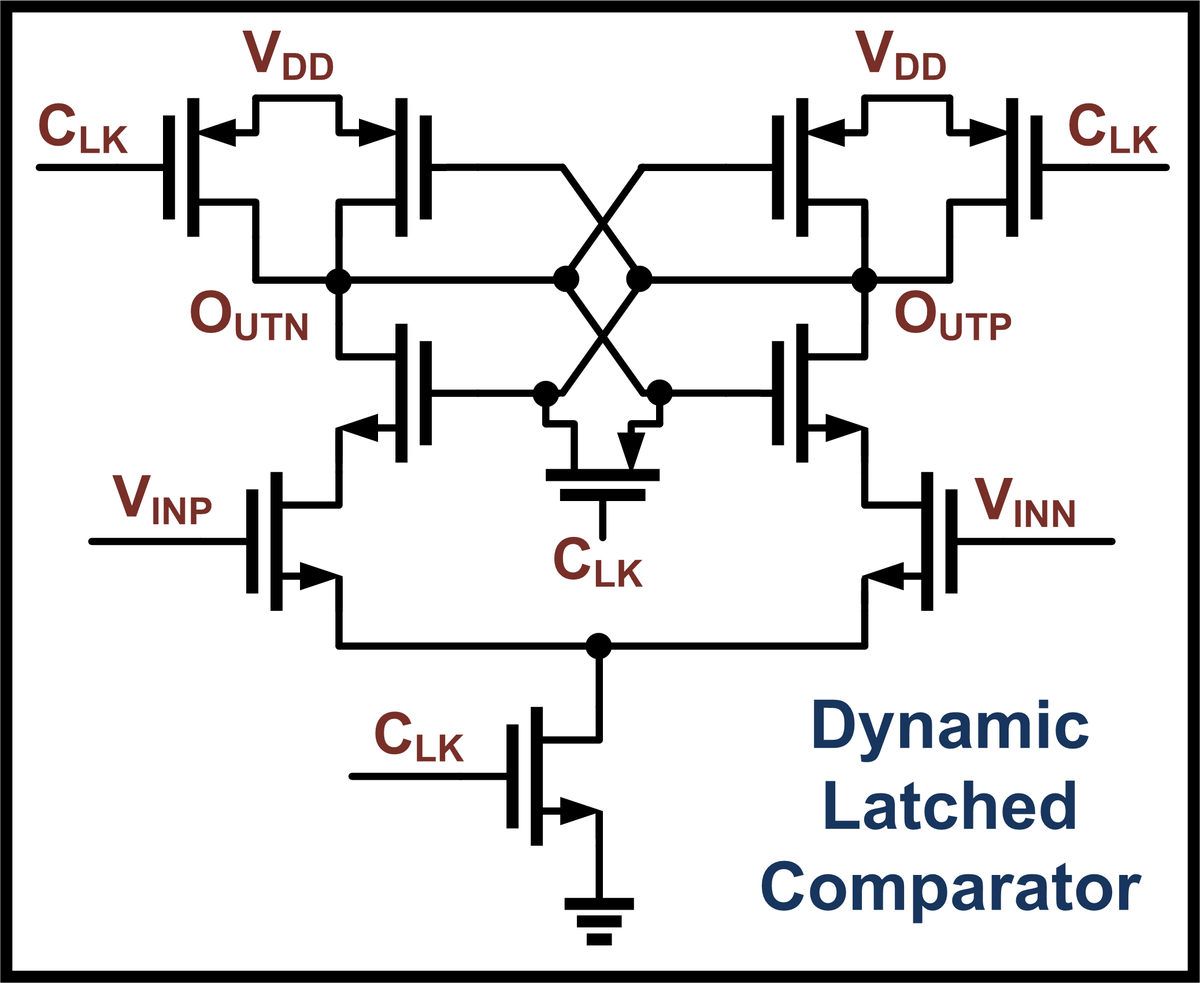
\includegraphics[scale = 1.8]{figures/Portada.png}
  \end{center}
  \vspace{1 cm}
  \begin{center}
    {\large
      Memoria de prácticas%Insert document type (e.g., Project Report)
    }\\
    \vspace{0.2cm}
    {\Large \begin{center}
      Alejandro Gómez Gambín \space \space \space \space Pablo Martínez Sánchez
      \newline /GTE3B%Insert your group name or real names here
      \end{center}
    
    }
  \end{center}
  \vfill
  \begin{center}
  Universidad Politécnica de Valencia\\
  Fundamentos de VLSI
  \end{center}
\end{titlepage}
\clearpage
\thispagestyle{empty}
\pagenumbering{roman} %use roman page numbering in the frontmatter
{\small
\strut\vfill % push the content to the bottom of the page
\noindent Copyright \copyright{} Universidad Politécnica de Valencia\par
\vspace{0.2cm}
\noindent Este informe se ha realizado con el editor \url{www.overleaf.com} en su versión gratuita con la ayuda de la guía \cite{Guide} y el foro \cite{Stack}. Las capturas de pantalla tomadas pertenecen al entorno de diseño Cadence, ejecutado sobre una máquina virtual de Linux alojada en PoliLabs.
}
\clearpage
\pdfbookmark[0]{English title page}{label:titlepage_en}
\pagenumbering{roman} %use roman page numbering in the frontmatter
\aautitlepage{%
  \englishprojectinfo{
  Análisis y Dimensionado de un Circuito CMOS Dinámico %title
  }{%
    Diseño y simulación de Esquemáticos en Entorno Cadence %theme
  }{%
    2º cuatrimestre, 3er año del GTSIT %project period
  }{%
    GTE3B % project group
  }{%
    %list of group members
    Alejandro Gómez Gambín\\
    Pablo Martínez Sánchez
    
  }{%
    %list of supervisors
    Miguel Ángel Larrea Torres
  }{%
    1 % number of printed copies
  }{%
    \today % date of completion
  }%
}{%department and address
  \textbf{Fundamentos de VLSI}\\
  Universidad Politécnica de Valencia\\
  \href{http://www.upv.es}{http://www.upv.es}
}
{\begin{itemize}
    \item Profundizar en el diseño jerárquico y en la captura de esquemas digitales en el entorno de trabajo Cadence.
    \item Comprender el funcionamiento de los circuitos combinacionales dinámicos.
    \item Comprender el dimensionado de transistores asociado al del reloj y la disposición en cascada de etapas y secciones dinámicas.
    \item Entender el funcionamiento de la Lógica Dinámica N y el por qué de la conexión entre etapas.
\end{itemize}
}


\pdfbookmark[0]{Contents}{label:contents}
\pagestyle{fancy} %enable headers and footers again
\tableofcontents
\noindent\hrulefill

ME LA SUDAAAAAAAAAAAAAAAAAAAAAAAA, LA PUPE ESTÁ ACOBARDADA, ES UNA CANSINA DE CUIDAO, VOY A POR ELLA EN VERANO A SU PUEBLO, AUNQUE SEA LA MAS PERRAAAAAAA, OH SHOULD I LEAVE? THINK SO, BYE

\cleardoublepage
\phantomsection
\listoffigures
\noindent\hrulefill
%mainmatter
\pagenumbering{arabic} %use arabic page numbering in the mainmatter

\renewcommand{\chaptername}{Sección}
\chapter{Introducción}

Esta memoria cubre todos los aspectos trabajados durante la Práctica 3 \cite{Guion} de la asignatura Fundamentos de VLSI. En ella, se incluye el proceso seguido para diseñar un Circuito de Lógica CMOS \cite{MOSFET} Dinámica y la simulación del esquemático que lo representa para responder a las cuestiones que se plantean en el guion de la práctica. La memoria se divide en las siguientes partes:

\begin{enumerate}
    \item \textbf{Síntesis de un Circuito CMOS Dinámico:} Se detalla el funcionamiento del circuito, las consideraciones a tener en cuenta a la hora del diseño, el esquemático del circuito y varios análisis transitorios, algunos de ellos paramétricos para hallar el dimensionado final del mismo. Este apartado se desarrollará en base a las 4 cuestiones que se plantean en la sección 2.2 del guion \cite{Guion}.
    \item \textbf{Encadenado de etapas dinámicas}: Incluye un esquemático en el que se encadenan y estimulan adecuadamente dos etapas del circuito CMOS dinámico diseñado previamente y un análisis transitorio del mismo. Este apartado se usará también para comentar por qué se ha de seguir un procedimiento específico a la hora de encadenar este tipo de circuitos.
    \item \textbf{Conclusiones:} Apartado donde se exponen de forma ordenada, las conclusiones a las que se ha llegado durante la realización de la práctica así como comentarios adicionales que merezca la pena realizar.
\end{enumerate}

Prueba de escritura GitHub

\begin{mylisting}[hbox,enhanced,drop shadow]{Java Program}
class MyClass
public static void main
\end{mylisting}

\newgeometry{top=0.5cm}
\renewcommand{\chaptername}{Sección}
\chapter{Síntesis de un Circuito Dinámico}\label{ch:ch2label}
\section{Definición del circuito}
\subsection{Lógica CMOS Dinámica}
Este tipo de lógica pretende reducir el área de la lógica CMOS convencional (simplificando el layout en consecuencia) evitando las desventajas de una lógica estática tales como el consumo en estado estacionario o la degradación de niveles lógicos.
\newline Esto se consigue aprovechando el hecho de que existen muchas señales en un circuito que no es necesario estar generándolas durante todo el ciclo de reloj, es decir, que se mantengan válidas durante todo el mismo sino sólo en determinados momentos.
\newline El principio de operación se basa en sustituir los transistores pMOS del plano P por un único pMOS gobernado por un reloj y añadir un nMOS adicional gobernado por el mismo reloj. Al eliminar la red P casi en su totalidad, se nos permite reducir casi a la mitad el área ocupada con la bajada en la potencia de disipada que ello conlleva.
\newline Este tipo de circuitos se pueden resumir en el siguiente esquema \cite{TheoryImages}:
\begin{figure}[h]%[!ht]
\begin{center}
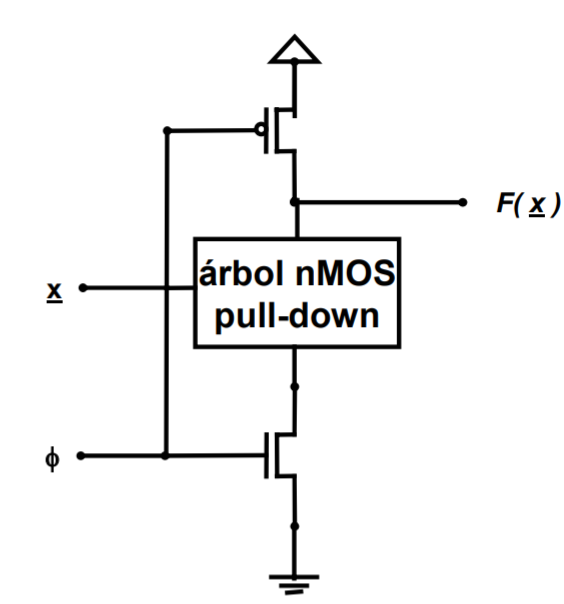
\includegraphics[width=0.5\textwidth]{figures/DynamicBasic.PNG}
\caption{Esquema general de un circuito CMOS de lógica dinámica}
\label{fig:DynBasic}
\end{center}
\end{figure}
\newline Donde \textit{X} serían las entradas de la puerta lógica y $\phi$ el reloj que gobierna los dos transistores comentados previamente.
\newgeometry{top=3cm, bottom=2cm}
\par Se tendrían dos fases diferenciadas:
\begin{enumerate}
    \item \textbf{Precarga:} El nodo de salida se carga a un valor lógico incondicionalmente mientras la red de evaluación permanece desconectada.
    \item \textbf{Evaluación:} La red de evaluación puede alterar el valor del nodo de salida.
\end{enumerate}
\begin{figure}[h]%[!ht]
\begin{center}
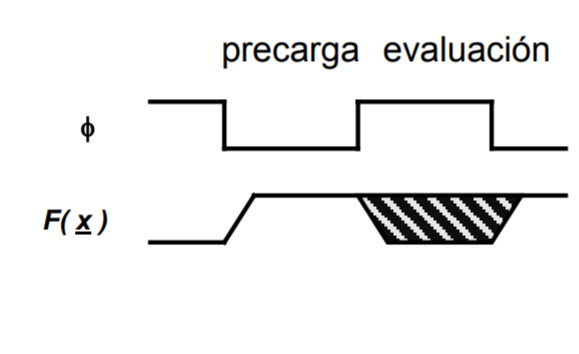
\includegraphics[width=0.4\textwidth]{figures/DynamicGraph.PNG}
\caption{Fases de un circuito CMOS dinámico}
\label{fig:Ib}
\end{center}
\end{figure}
\par \cite{TheoryExpl} En primer lugar, cuando el reloj ($\phi$) es cero, el nodo de salida de la puerta se lleva a nivel alto y será el transistor pMOS el que conducirá, lo que cargará en la salida un 1. Cuando $\phi$ se ponga a uno, en función de las entradas, la salida se quedará con el uno que tenía ya la capacidad asociada al nudo de salida no tiene sitio por donde descargarse ó el nMOS inferior se encargará de descargar la salida, dejando un cero. Además, hay que tener en cuenta que, durante la evaluación se pueden producir fugas de carga que descarguen el nodo a la salida.

\par Sin embargo, estos circuitos tienen problemas evidentes como su sensibilidad al ruido o el consumo asociado al reloj que puede llegar a ser muy elevado.
\subsection{Lógica Dominó}
Otro de los problemas de esta lógica es el encadenar etapas. El conflicto con este tipo de circuito radica en que puede ocurrir que una puerta sea algo más rápida que las anteriores y darle tiempo a evaluar mientras que las anteriores se encuentran todavía en fase de precarga. Para solucionar esto se emplea lo que se llama lógica dominó.
\begin{figure}[H]%[!ht]
\begin {center}
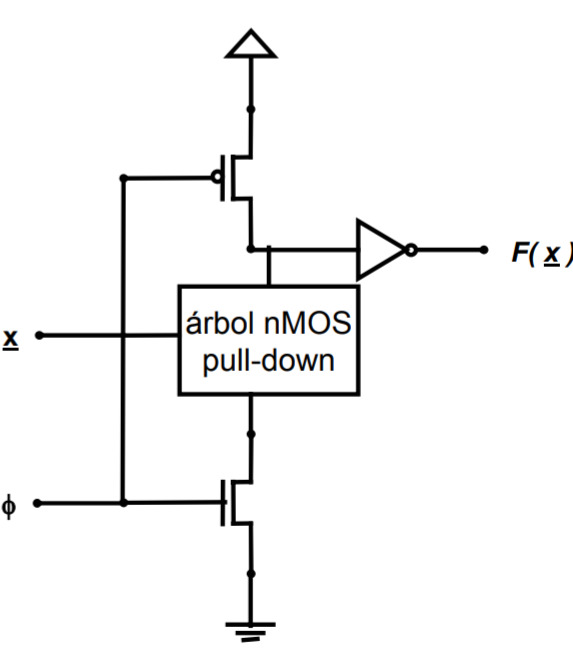
\includegraphics[width=0.4\textwidth]{figures/DominoBasic.PNG}
\caption{Esquemático básico de la Lógica Dominó}
\label{fig:Dominobasic}
\end {center}
\end{figure}
Como se puede observar, con la adición de un inversor CMOS a la salida, durante la fase de precarga se ataca a las siguientes etapas con ceros y aunque la evaluación de una puerta se atrase, ello sólo introduce un pequeño retraso en la evaluación definitiva pero no un error irreversible ya que la carga del nodo precargado no se puede disipar porque hasta que no se produzca la evaluación de las puertas anteriores, los transistores nMOS no conducen. (Esta es la razón por la que se le da el nombre de dominó, las primeras etapas determinan si las siguientes caen o no como piezas de dominó). 
\begin{figure}[h]%[!ht]
\begin {center}
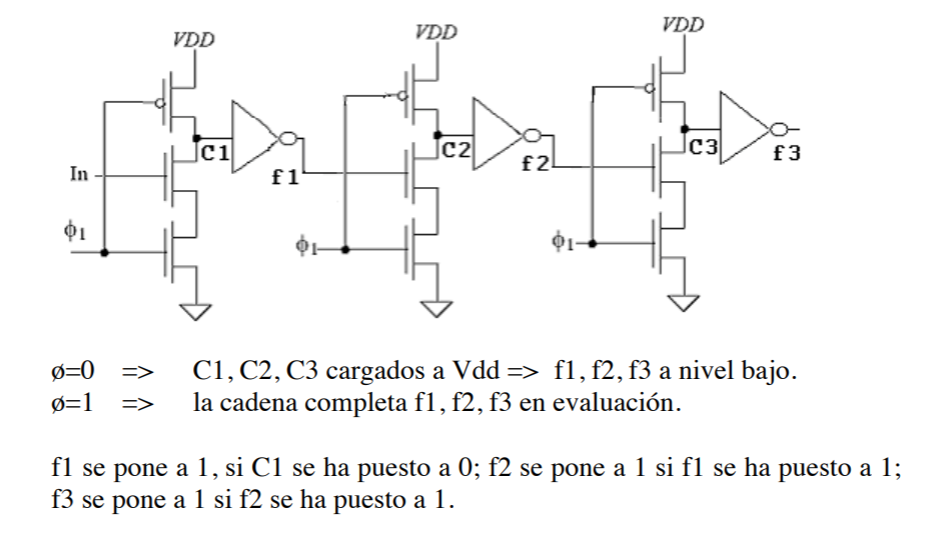
\includegraphics[width=1\textwidth]{figures/DominoEnc.PNG}
\caption{Encadenamiento de etapas con Lógica Dominó}
\label{fig:DominoEnc}
\end {center}
\end{figure} \newline
Con este esquema te aseguras de que todas las entradas son 0 durante la precarga lo que garantiza una única transición en las entradas (de 0 a 1) y reduce la capacidad del nodo de salida lo que facilita muy altas velocidades. \cite{TheoryAdvant}
\newline Sin embargo, estas puertas lógicas son únicamente no inversoras debido al inversor de la salida.
\subsection{Especificaciones}
Para esta práctica se dimensionarán los transistores con su longitud de canal mínima permitida por la tecnología AMS utilizada $0.35\mu m$ y su ancho de puerta mínimo $0.4\mu m$ para reducir las capacidades de entrada. La tensión de alimentación será la correspondiente a la tecnología MOS (3.3V).
\newline Para los transistores PMOS superior y nMOS inferior que controlarán la carga y descarga del nodo de salida, se emplearán $W_E = 1\mu m$ (nMOS) y $W_P =0.4\cdot W_E = 0.4\mu m$. La relación entre ambos anchos se mantendrá a lo largo de toda la práctica pero, en al final de esta sección se hará un análisis paramétrico de este parámetro. \newpage
\par Dicho esto, las cuestiones planteadas en el guion y que se irán respondiendo a lo largo de esta sección son las siguientes:
\begin{enumerate}
    \item ¿Qué Tipo de Lógica Dinámica es y qué Función Combinacional realiza?.
    \item ¿Qué porcentajes del Periodo de Reloj asignaría, en principio, a la Precarga y a la Evaluación?.
    \item Con los valores iniciales de WP y WE…. ¿Cuál es el valor máximo de la frecuencia Freq de Clock, supuesto el reloj simétrico, con tiempos fijos $t_{rise} = t_{fall} = 0.1 ns$?.
    \item Tomando $W_E$ como variable. ¿Cuál es su valor mínimo para operar a 500 MHz, con $t_{rise} = t_{fall} = 0.1 ns$?.
\end{enumerate}

\section{Captura del diseño}
Una vez se han dado las especificaciones necesarias, se ha procedido a crear una CellView nueva utilizando el programa Schematics L incluido en el Entorno de Cadence donde se ha creado el esquemático. Este ha sido el resultado:

\begin{figure}[h]%[!ht]
\begin {center}
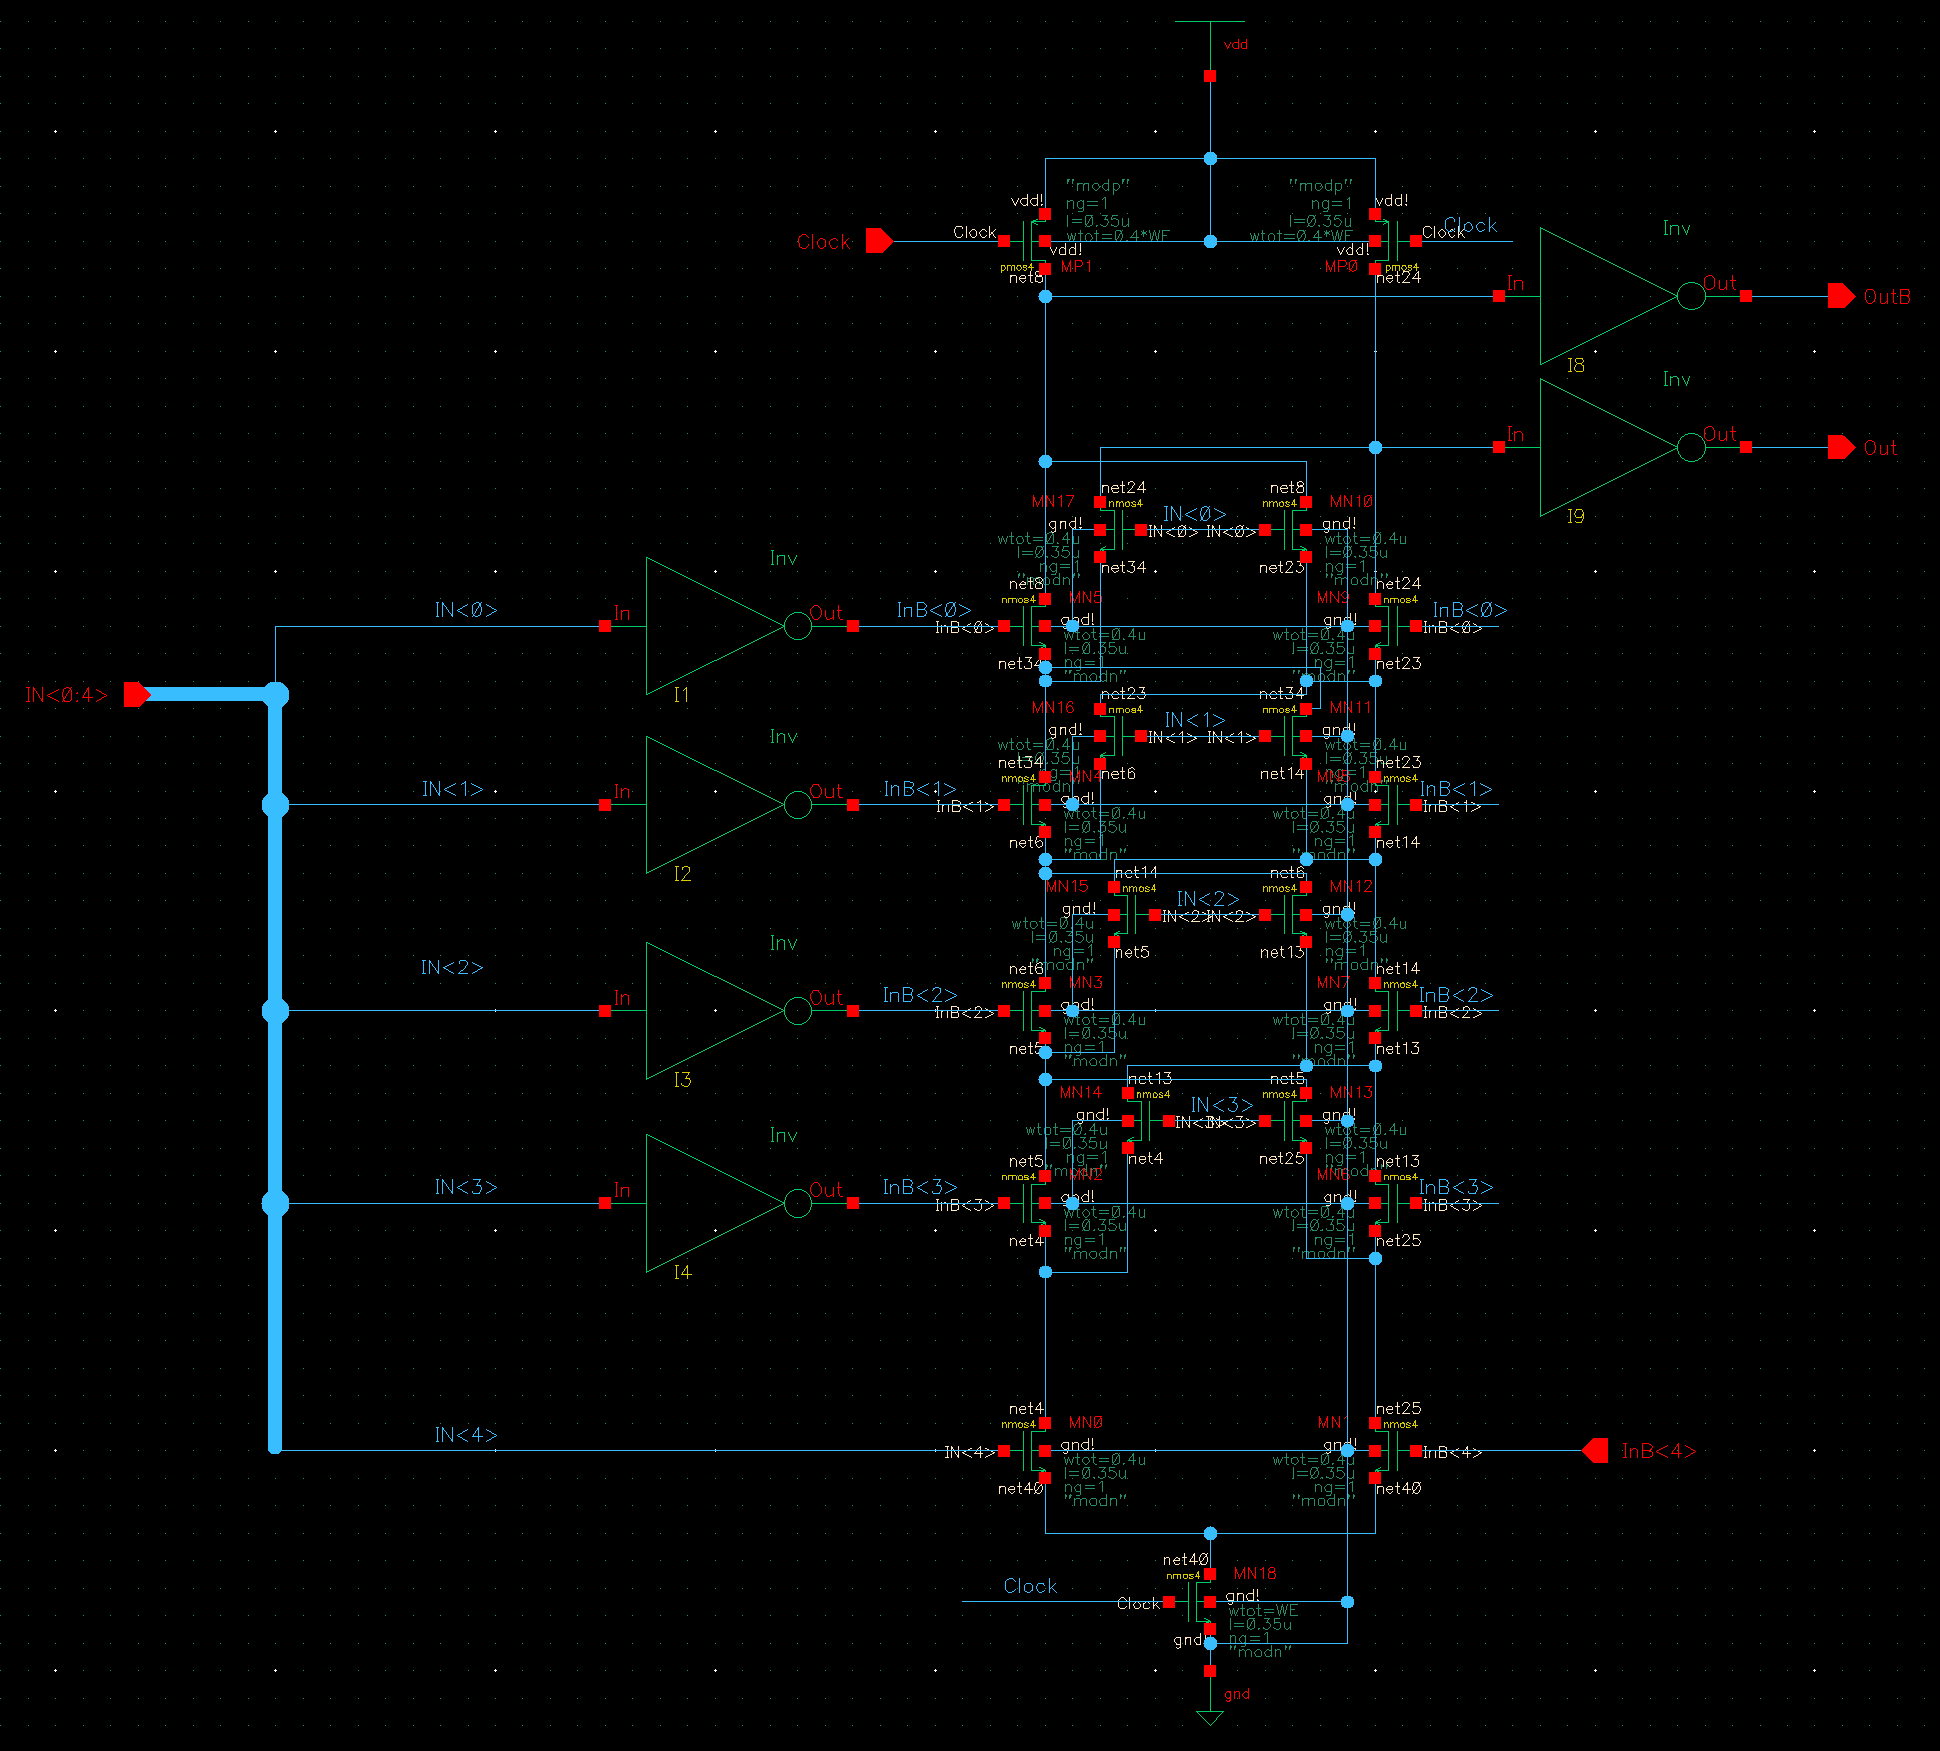
\includegraphics[width=1\textwidth]{figures/BlockDynSchem.PNG}
\caption{Esquema de la Etapa CMOS Dinámica (BlockDyn)}
\label{fig:BlockDynSchem}
\end {center}
\end{figure}
Se han utilizado los \textit{nmos4} y \textit{pmos4} de PRIMLIB, perteneciente a la tecnología \textbf{AMS TECH\_C35B4}. Además, se han utilizado las tomas de alimentación y de masa (vdd y gnd) pertenecientes a la librería analogLib, que es tecnoindependiente. \newline
Se ha introducido un parámetro, que esta vez no lo tomaremos como CDF sino que le daremos un valor en el ADE posteriormente para propósitos de simulación.
En cuanto a las dimensiones de los transistores, la longitud de canal es la mínima ($0.35\mu m$) y el ancho depende del tipo de MOS: como la movilidad de los electrones (portadores negativos) es 2.5 veces superior a la de los huecos (portadores positivos), el ancho del canal del NMOS se toma como el mínimo ($0.4\mu m$) y el ancho del PMOS es 2.5 veces mayor ($1\mu m$), como ya se ha comentado en las especificaciones.
\par Como el esquemático tiene tantos transistores, se ha decidido tomar la idea que aparece en el guion de incluir capturas de pantalla con un zoom sobre determinadas partes del esquemático:
\begin{figure}[h]%[!ht]
\begin{center}
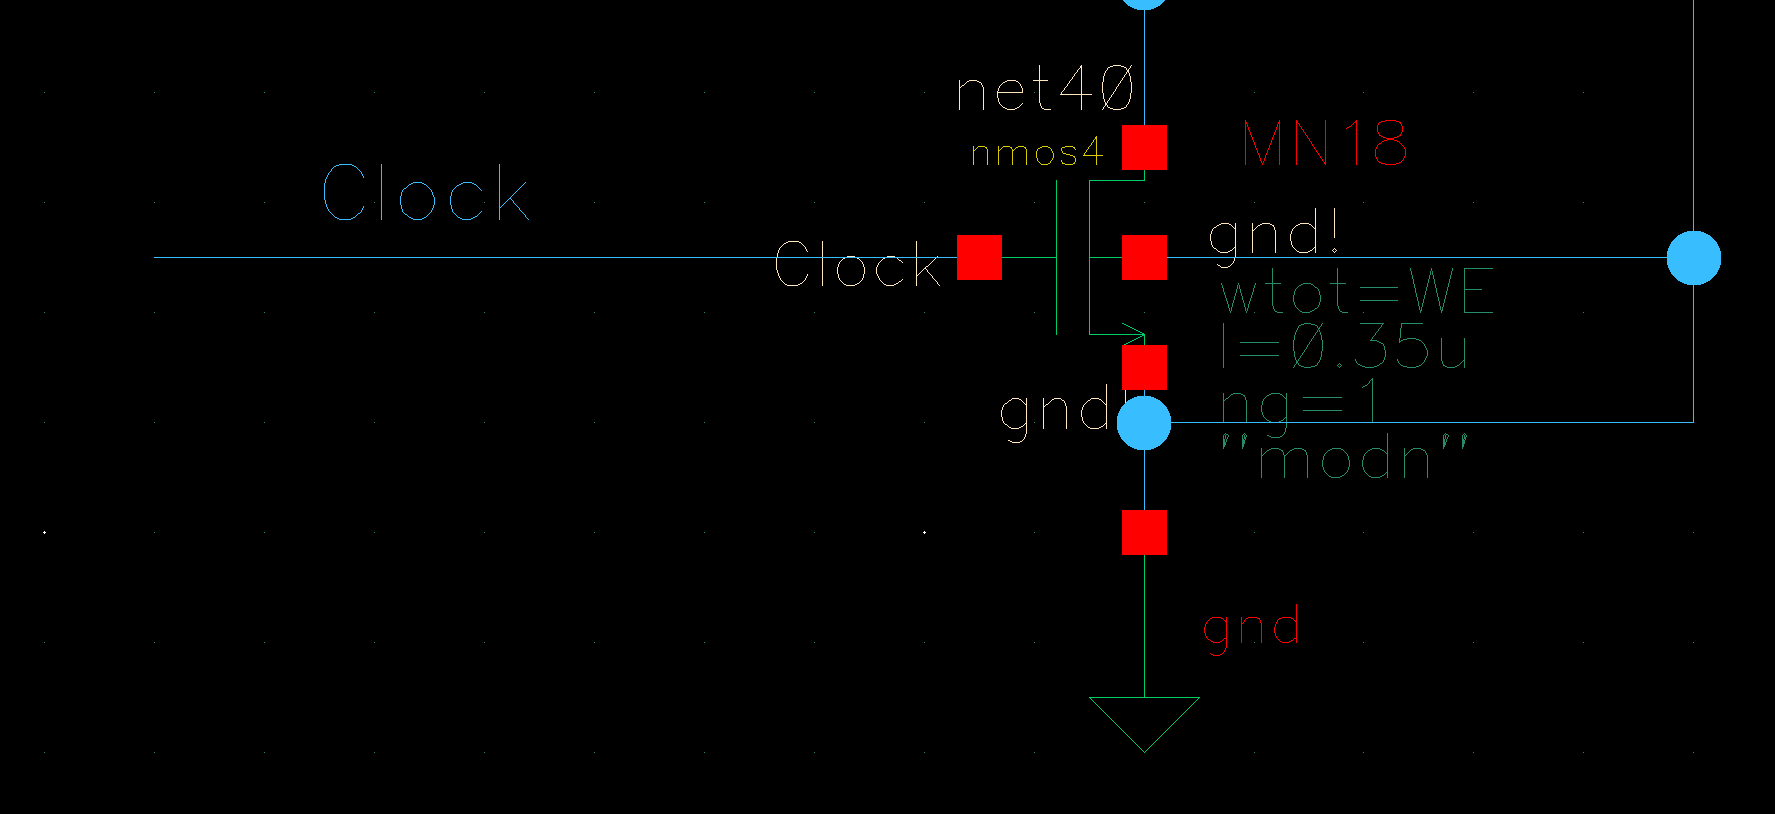
\includegraphics[width=0.8\textwidth]{figures/DeatilNMOS.PNG}
\label{fig:CDF}
\end{center}
\end{figure}
\begin{figure}[h]%[!ht]
\begin{center}
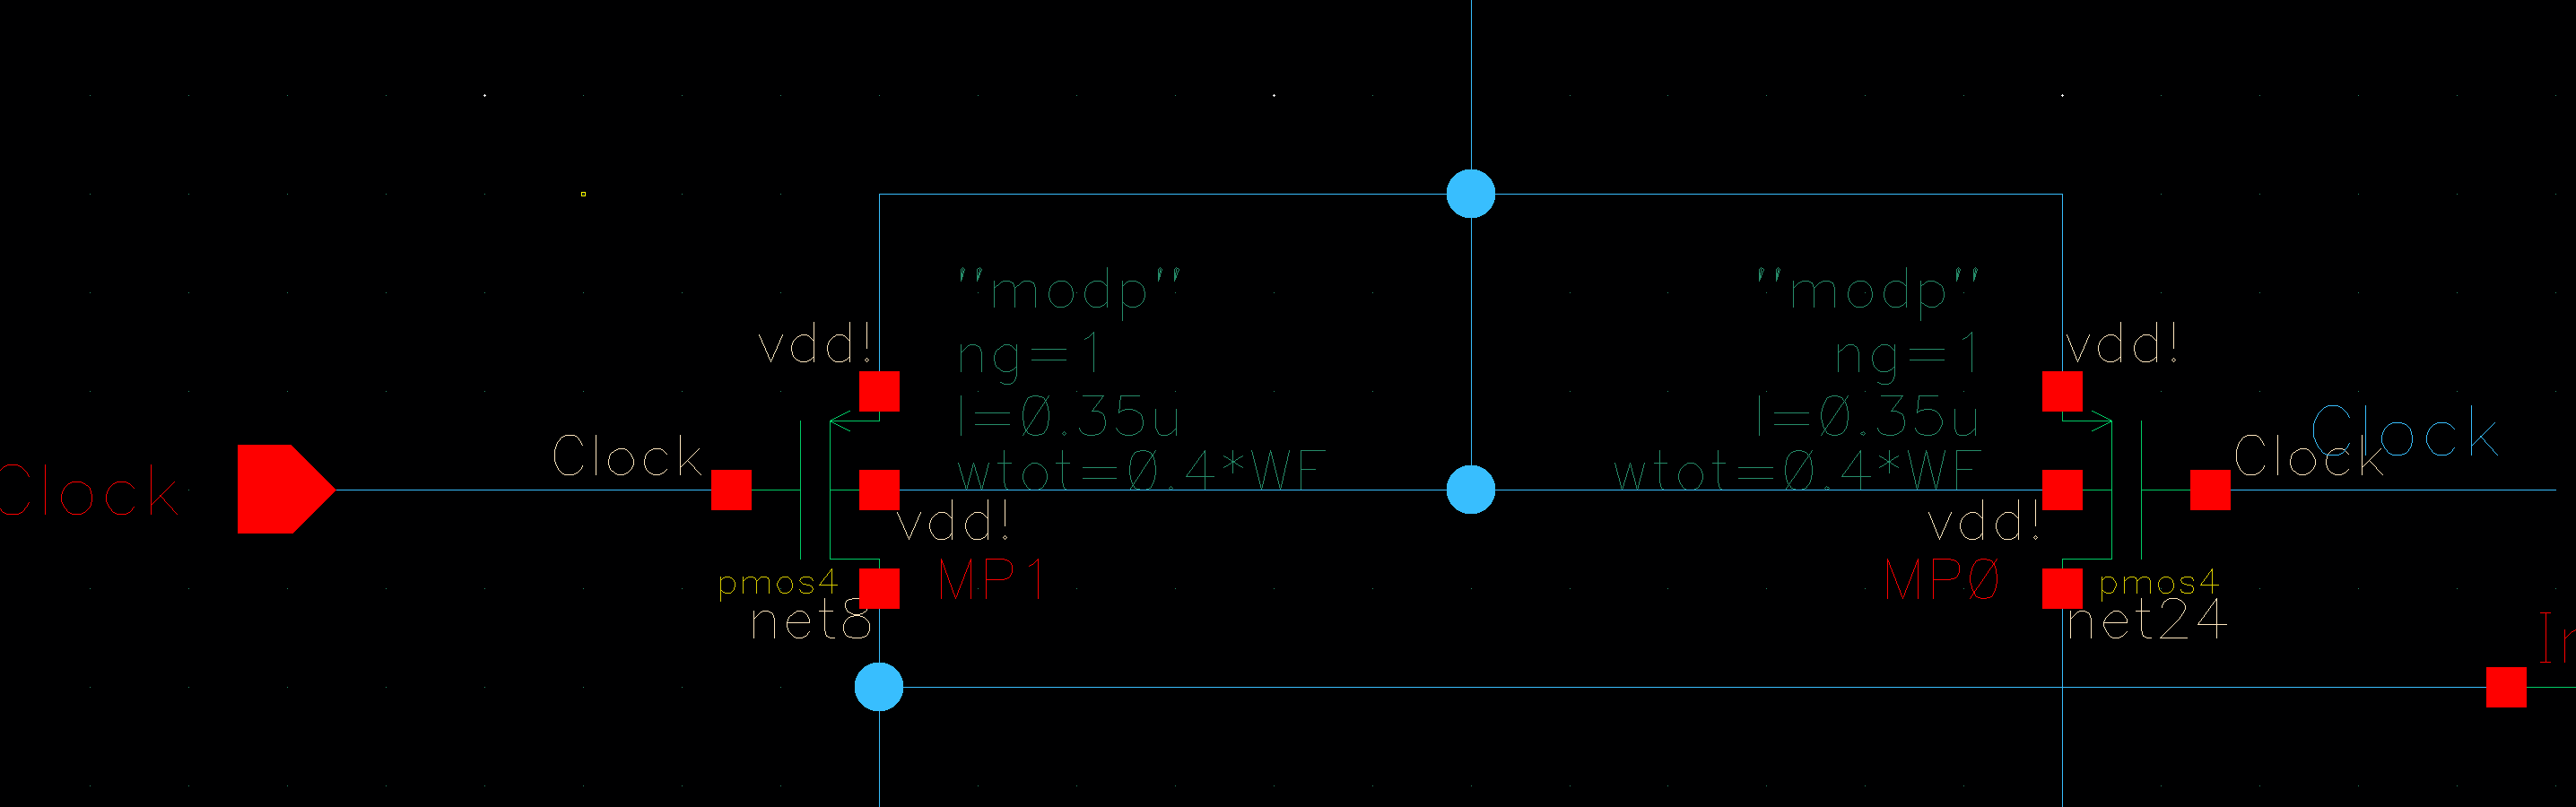
\includegraphics[width=0.8\textwidth]{figures/DetailPMOS.PNG}
\caption{Vista en detalle del pMOS de precarga y el NMOS de descarga de la red que ejecuta la función lógica}
\end{center}
\end{figure} \newline
En este esquemático se ha utilizado otra herramienta del Schematic Editor L de Cadence que serían los buses, que nos permiten hacer cables de varios bits de ancho a diferencia de Wire (Narrow) que sólo podía transportar un bit. Gracias a la conexión por nombre se han etiquetado los distintos bits que salían del bus y se han conectado \say{by name} a las puertas de la escalera central del esquemático. Los inversores utilizados pertenecen a la librería PIEZAS\_DIG, son en concreto la célula \textbf{Inv}.
\newline Si observamos la estructura del esquemático, el tipo de lógica dinámica que realiza es \textbf{dominó}, sólo hay que comparar el esquemático con la figura \ref{fig:Dominobasic} para darnos cuenta de que, aparte de cumplir con las características de un Circuito CMOS dinámico, presenta inversores en sus salidas. Además, hay un pMOS extra que precarga los nudos internos para solucionar el charge sharing.
\section{Simulaciones}
El resto de cuestiones quedarán respondidas tras haber realizado una simulación que dividiremos en tres etapas 
\subsection{Análisis transitorio inicial}
Se ha construido el testbench propuesto en el guion de la práctica:
\begin{figure}[h]%[!ht]
\begin{flushleft}
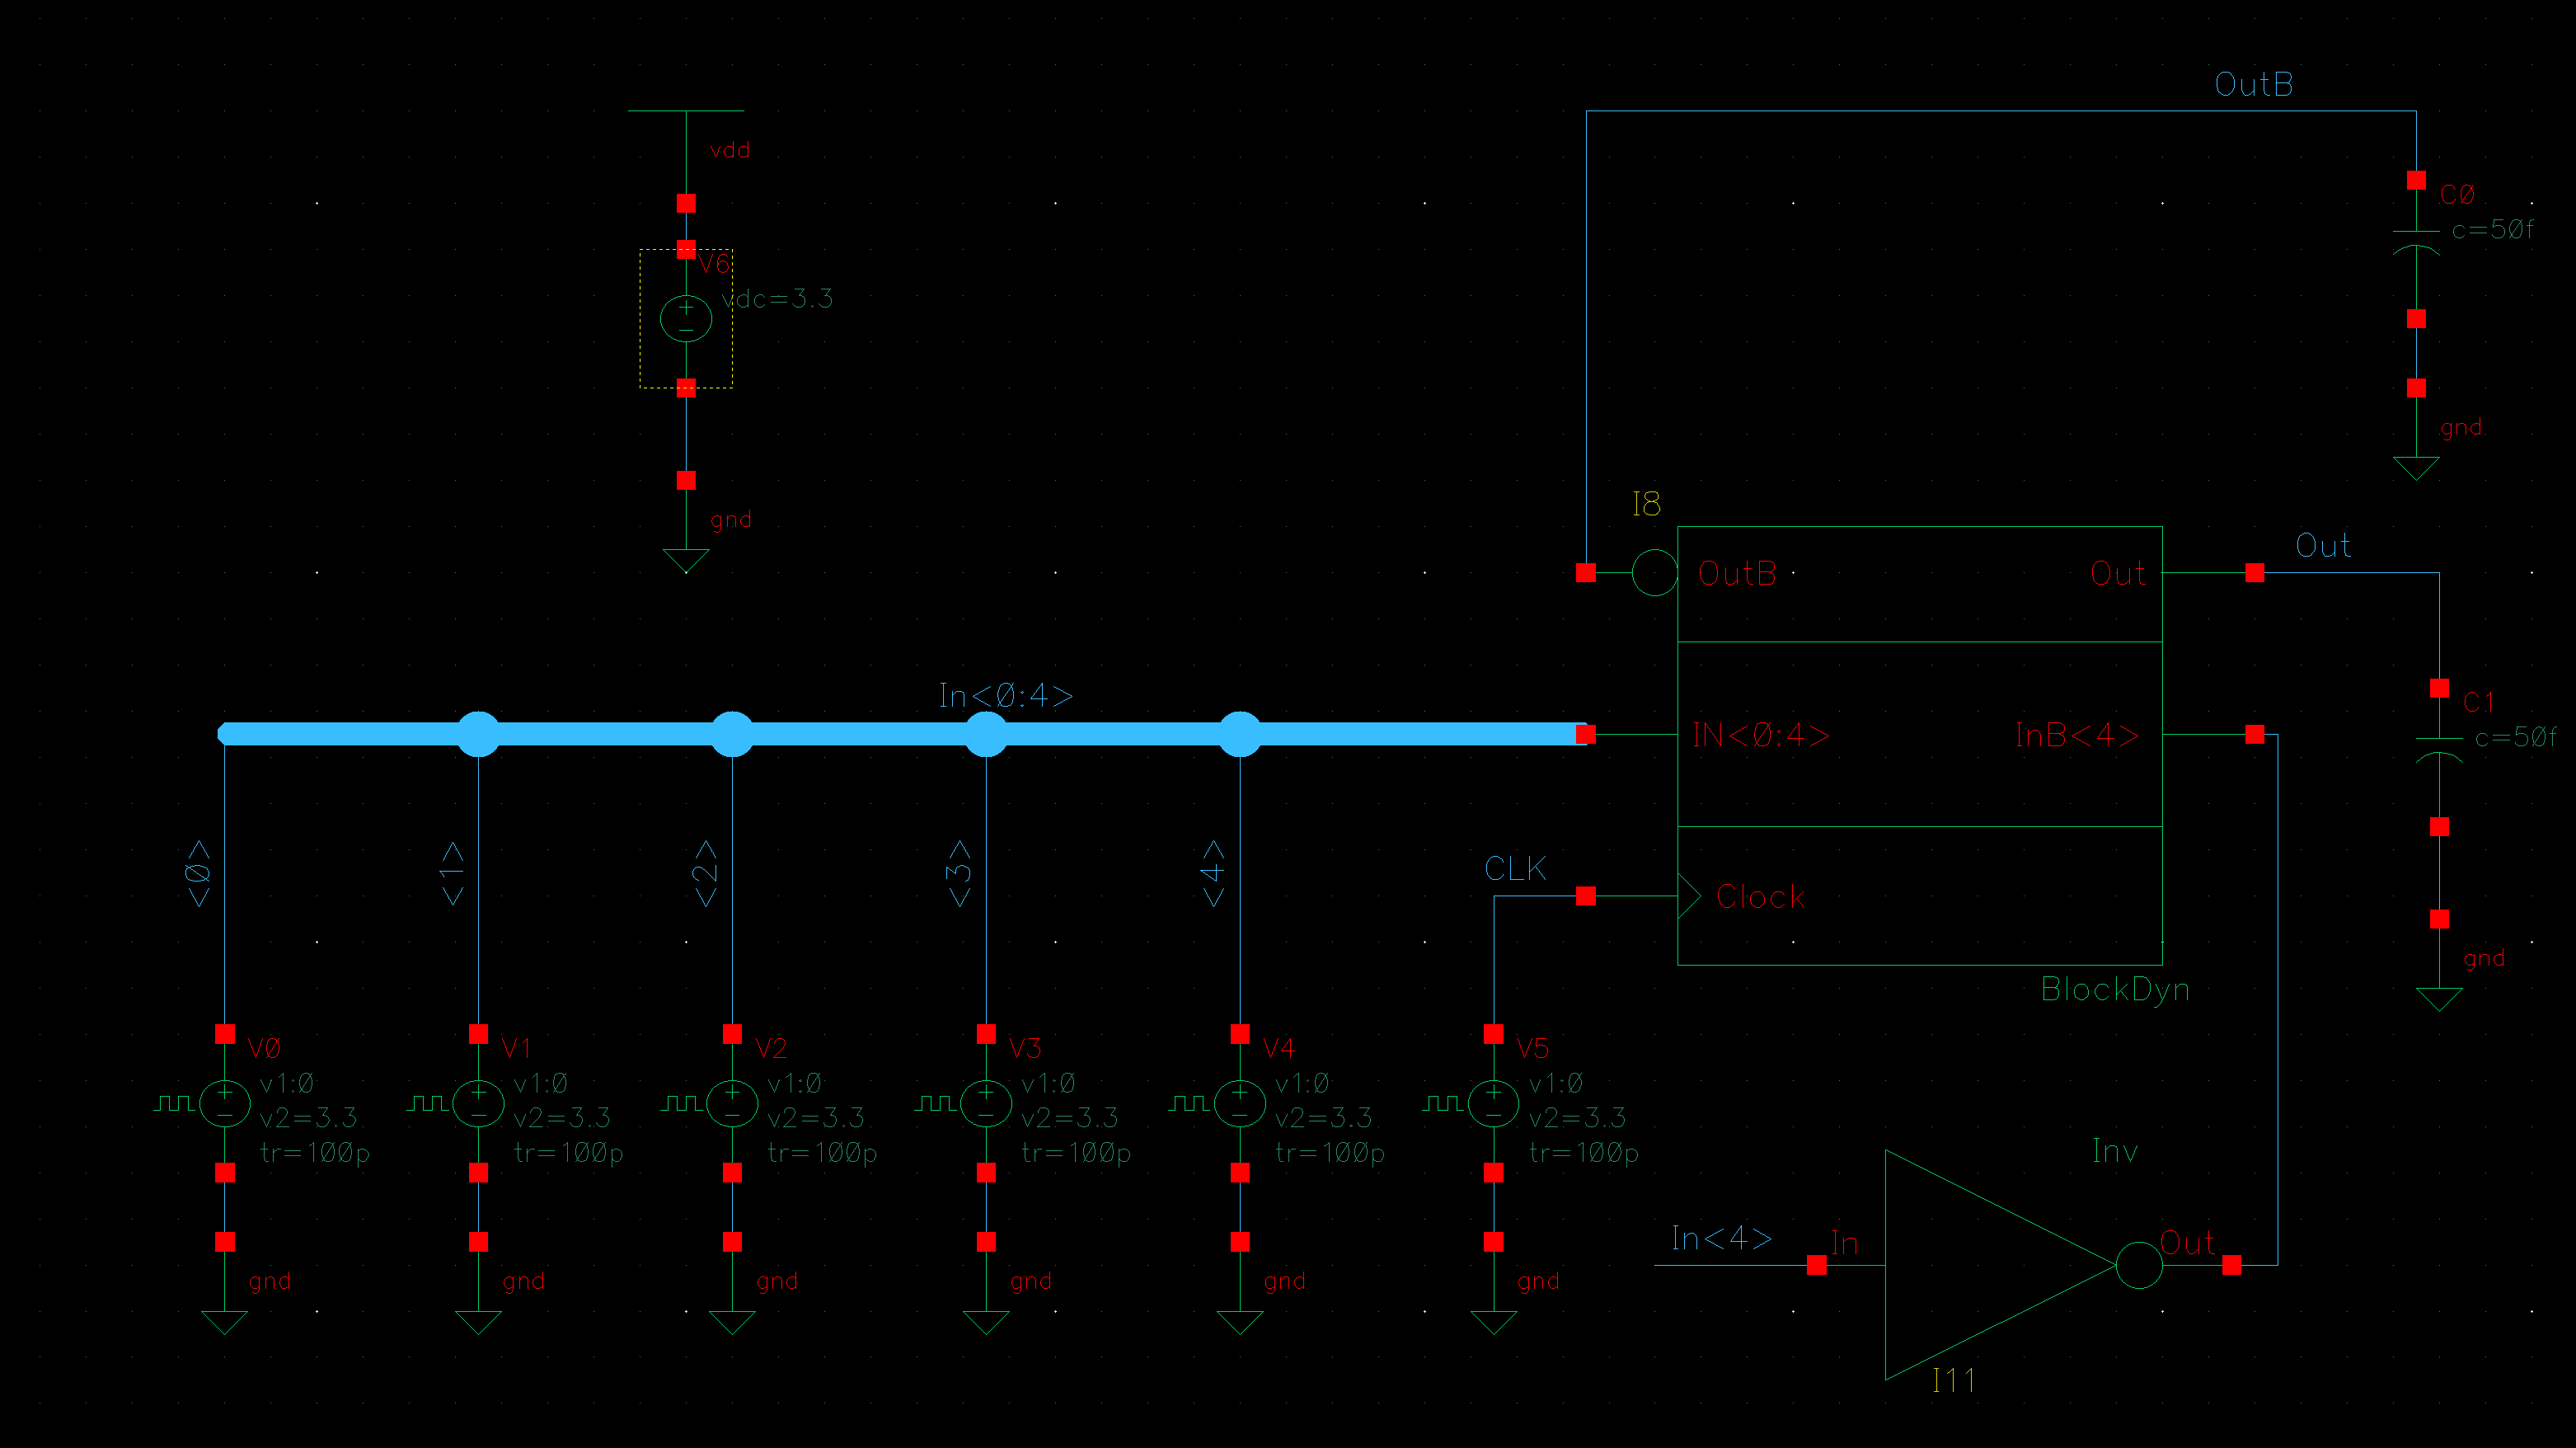
\includegraphics[width=1.1\textwidth]{figures/BlockDynTBSchem.PNG}
\caption{Banco de pruebas para BlockDyn}
\label{fig:BlockDynTBSchem}
\end{flushleft}
\end{figure} \newline
Donde se ha estimulado el circuito con un reloj de periodo \textit{TPeriod} parametrizable y simétrico y se han ido colocando señales cuadradas a cada entrada de forma que se reproduzcan todas las combinaciones posibles de entradas. 
\newpage Aquí se muestran como ejemplos In<1>, In<2>  e In<5>, de izquierda a derecha:
\begin{figure*}[h]
\begin{multicols}{3}
    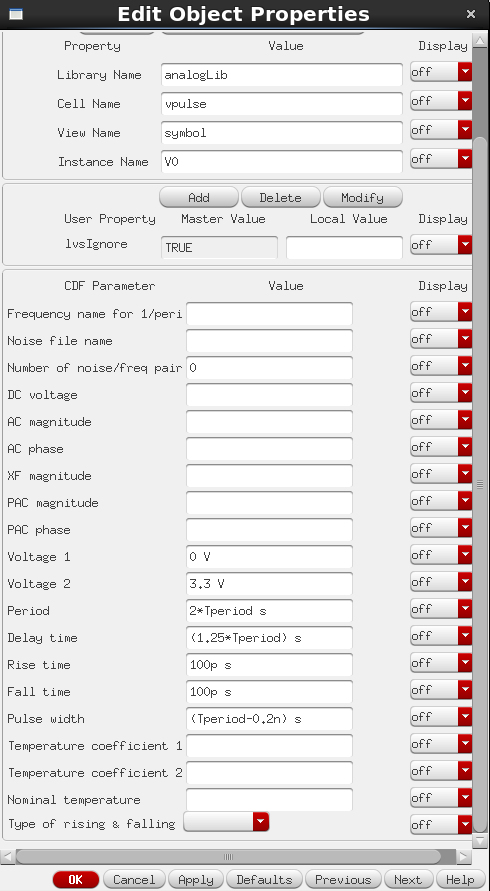
\includegraphics[width=1\linewidth]{figures/In1Config.PNG}\par 
    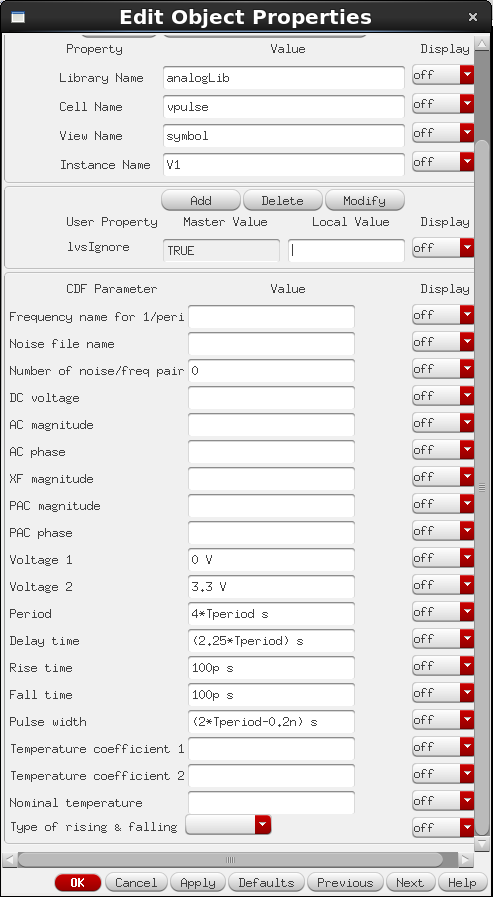
\includegraphics[width=1\linewidth]{figures/In2Config.PNG}\par
    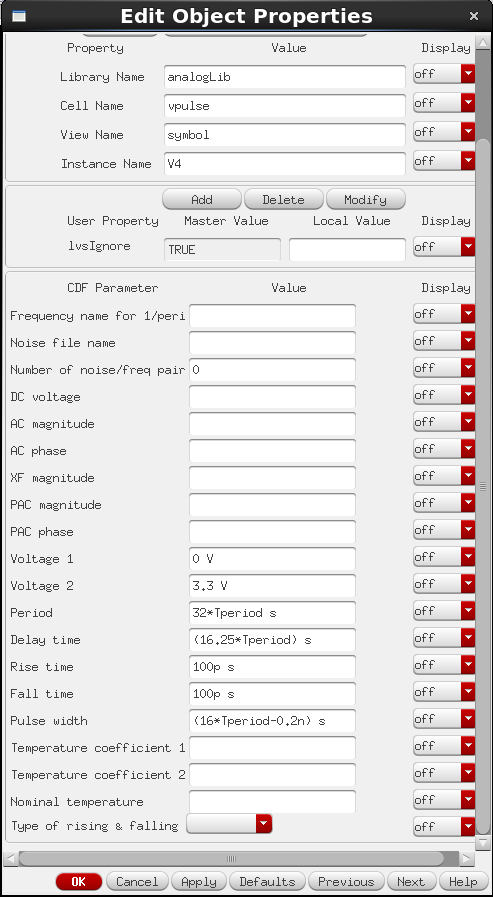
\includegraphics[width=1\linewidth]{figures/In4Config.PNG}\par 
    \end{multicols}
    \caption{Señales de entrada}
\end{figure*} \newline
Con este testbench, se ha abierto el Analog Design Environment L y se ha configurado el siguiente estado denominado \textit{state1}:
\begin{figure}[H]%[!ht]
\begin {center}
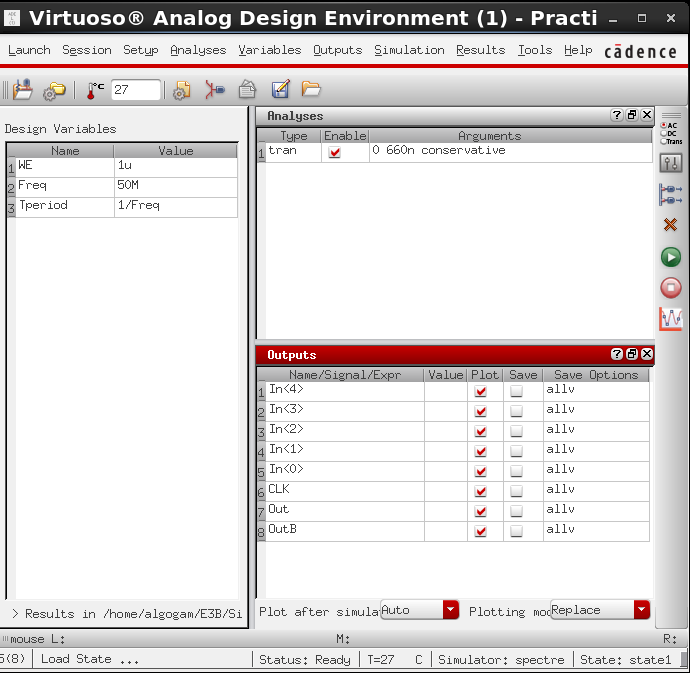
\includegraphics[width=0.6\textwidth]{figures/State1Config.PNG}
\caption{Estado con los valores iniciales de la simulación}
\label{fig:State1}
\end {center}
\end{figure} 

Donde se ha puesto, tal y como se propone en las especificaciones de la práctica se ha comenzado con una frecuencia de 50MHz y un ancho para los transistores de tipo N $1\mu m$.
\newpage Tras ejecutar la simulación, se obtuvo el siguiente resultado:
\begin{figure}[h]%[!ht]
\begin {center}
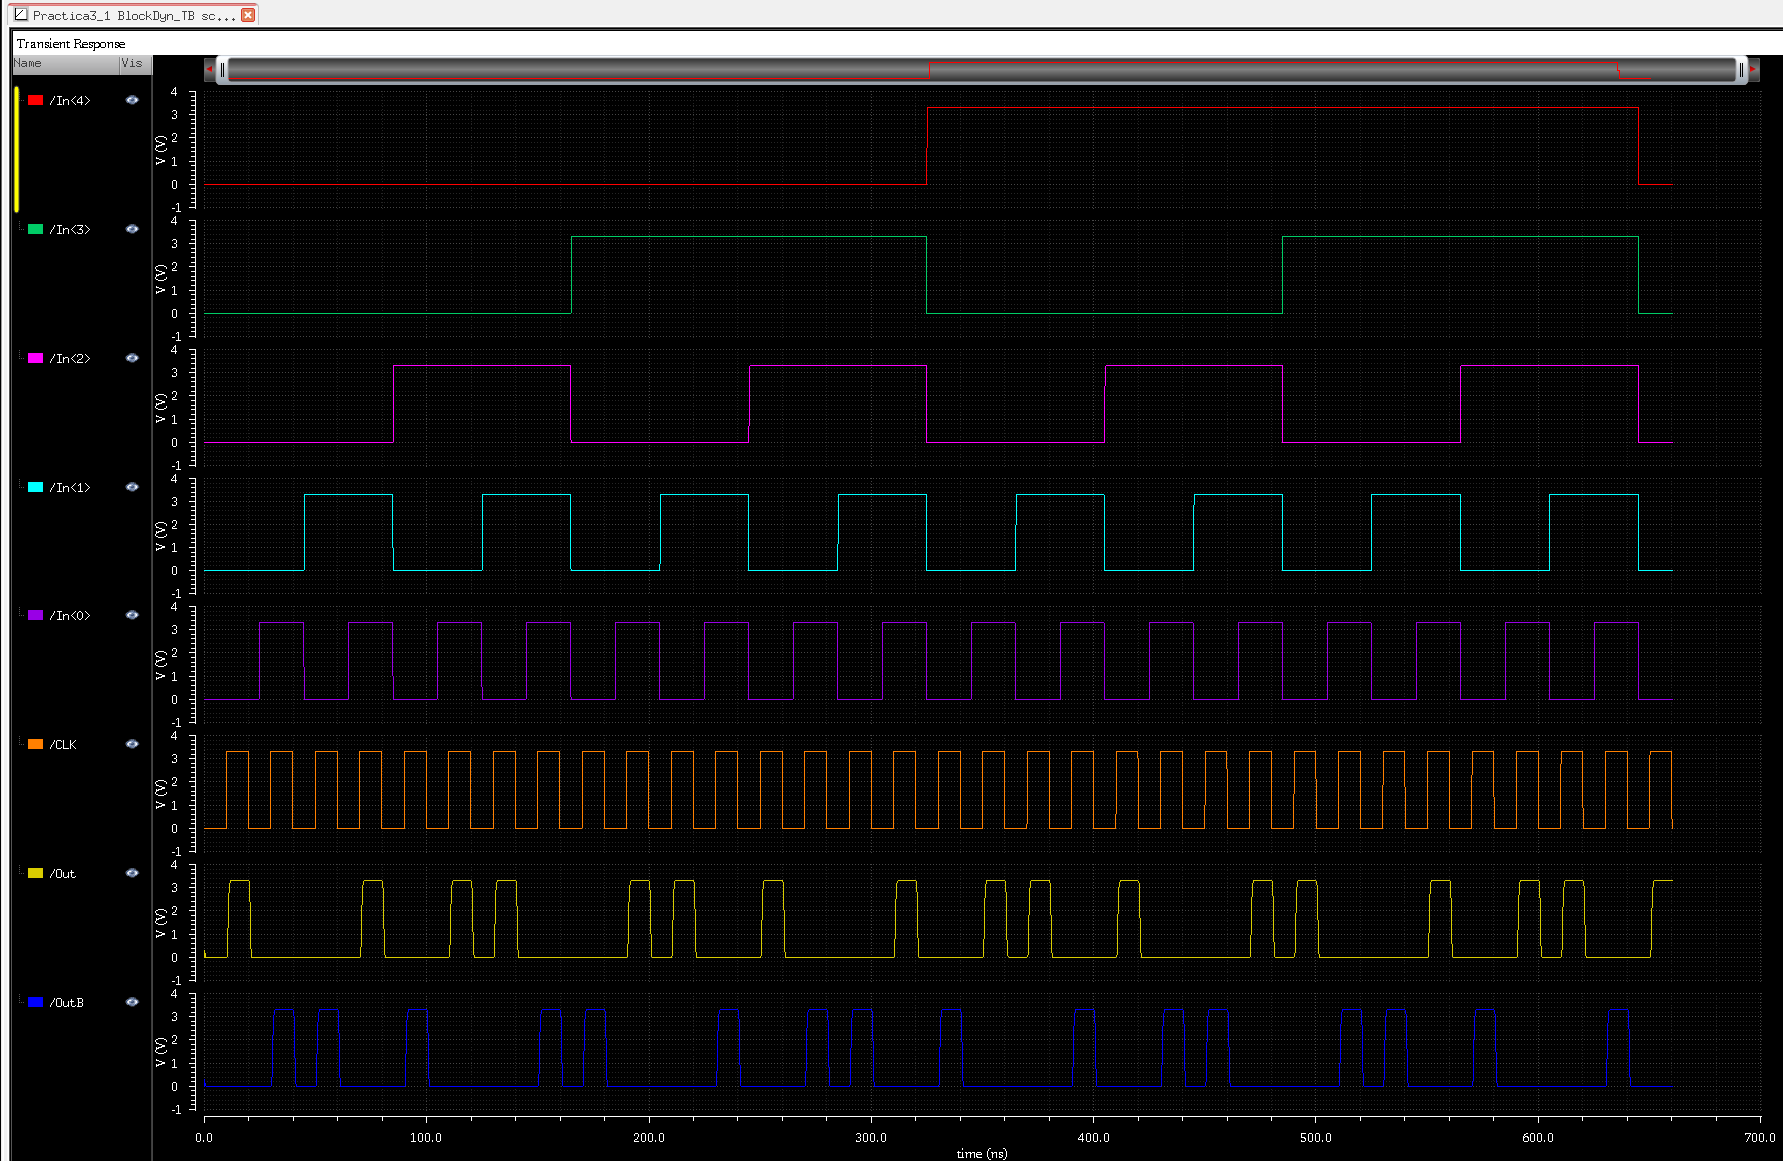
\includegraphics[width=1\textwidth]{figures/GraphState1TB.PNG}
\caption{Gráfica con los resultados de la simulación inicial}
\label{fig:GraphState1}
\end {center}
\end{figure} \newline
Si observamos atentamente las dos salidas vemos que OutB es la negada de Out pero sólamente cuando el reloj (traza naranja) vale 1. ¿Qué significa esto? Bien, esto es lógica CMOS dinámica, cuando el reloj está a cero, nos encontramos en la fase de precarga y al ser lógica dominó con un inversor a la salida, esta vale 0 en vez de 1 en la fase de precarga siempre, tanto para Out como OutB. En la fase de evaluación, si nos fijamos en las entradas vemos que sólamente cuando un número impar de ellas están a nivel alto, Out devuelve un 1 y, al contrario, cuando el número de unos es par, es OutB devuelve un 1, es decir, estamos ante un detector de paridad en la que Out es la señal de paridad Par y OutB la de paridad Impar.
\par En esta simulación se ha decidido poner el reloj simétrico pero no tiene por qué ser así ya que invertir la mitad de tiempo en la precarga cuando a lo mejor, por los tiempos de propagación, no es necesario darle todo ese tiempo para que el nudo de salida se ponga a uno.  Por lo tanto, sería mejor un mayor porcentaje del reloj a uno que a cero eso sí, teniendo en cuenta el retardo $t_{pmin}$ denotado en la figura 1 del guion \cite{Guion} y que, si dejamos demasiado tiempo el reloj a uno se pueden producir fugas demasiado grandes que degradarán el nivel de la señal de salida.  De la misma forma se debe respetar $t_{Emin}$ para que al circuito le dé tiempo a evaluar correctamente las entradas\newpage
\subsection{Análisis paramétrico con la frecuencia}
El siguiente paso es realizar un análisis en frecuencia con el valor de $W_E$ fijo para hallar cuál es la frecuencia máxima de operación a la cual este circuito sigue funcionando:
\begin{figure}[H]%[!ht]
\begin {center}
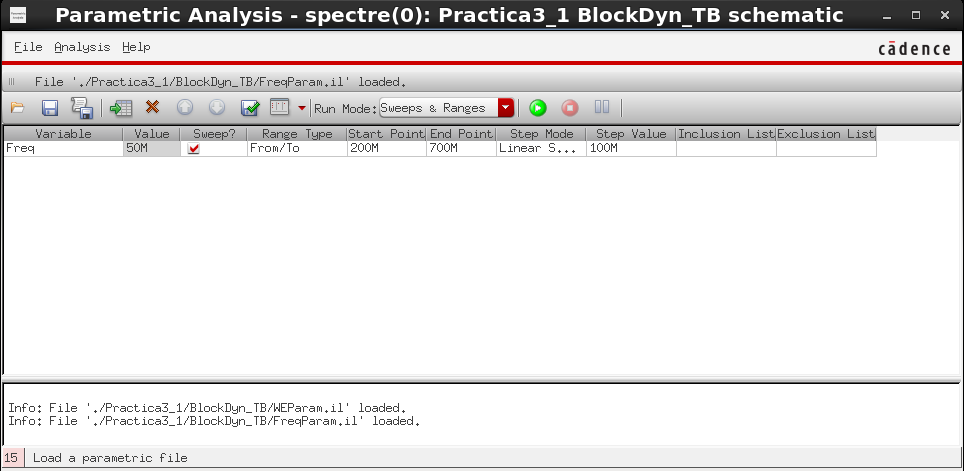
\includegraphics[width=1\textwidth]{figures/FreqParamConfig.PNG}
\caption{Configuración del análisis paramétrico en frecuencia}
\label{fig:ConfigFreqParam}
\end {center}
\end{figure} 
Además, se ha definido el siguiente estado, donde sólo se mostrarán las salidas y, además, se ha reducido el tiempo de simulación ya que las frecuencias altas tardan mucho en simular y las señales de salida son tan estrechas que no merecía la pena estar simulando durante tanto rato:
\begin{figure}[H]%[!ht]
\begin {center}
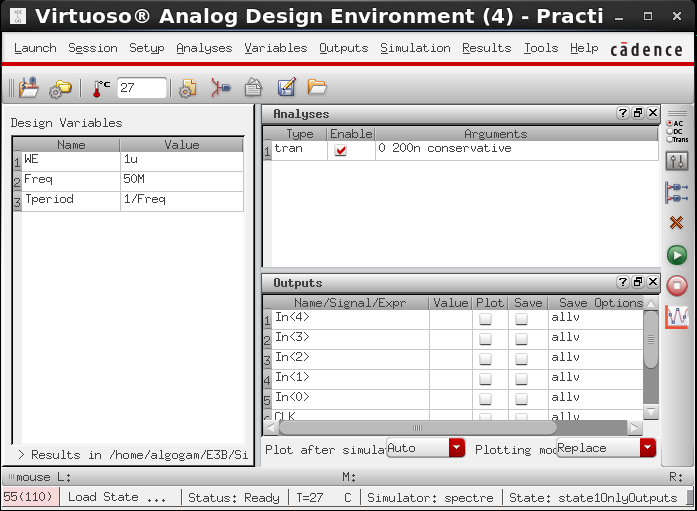
\includegraphics[width=0.85\textwidth]{figures/State1OnlyOutputsConfig.PNG}
\caption{Estado 1 con sólo las entradas}
\label{fig:ConfigState1OnlyOutputs}
\end {center}
\end{figure} 
Cabe destacar que se hicieron dos \say{Run} de la simulación, una desde 200MHz hasta 700MHz y otra desde 700MHz hasta 1.2GHz, algo excesivo pero con la intención de ver la evolución de la salida:
\begin{figure}[H]%[!ht]
\begin {center}
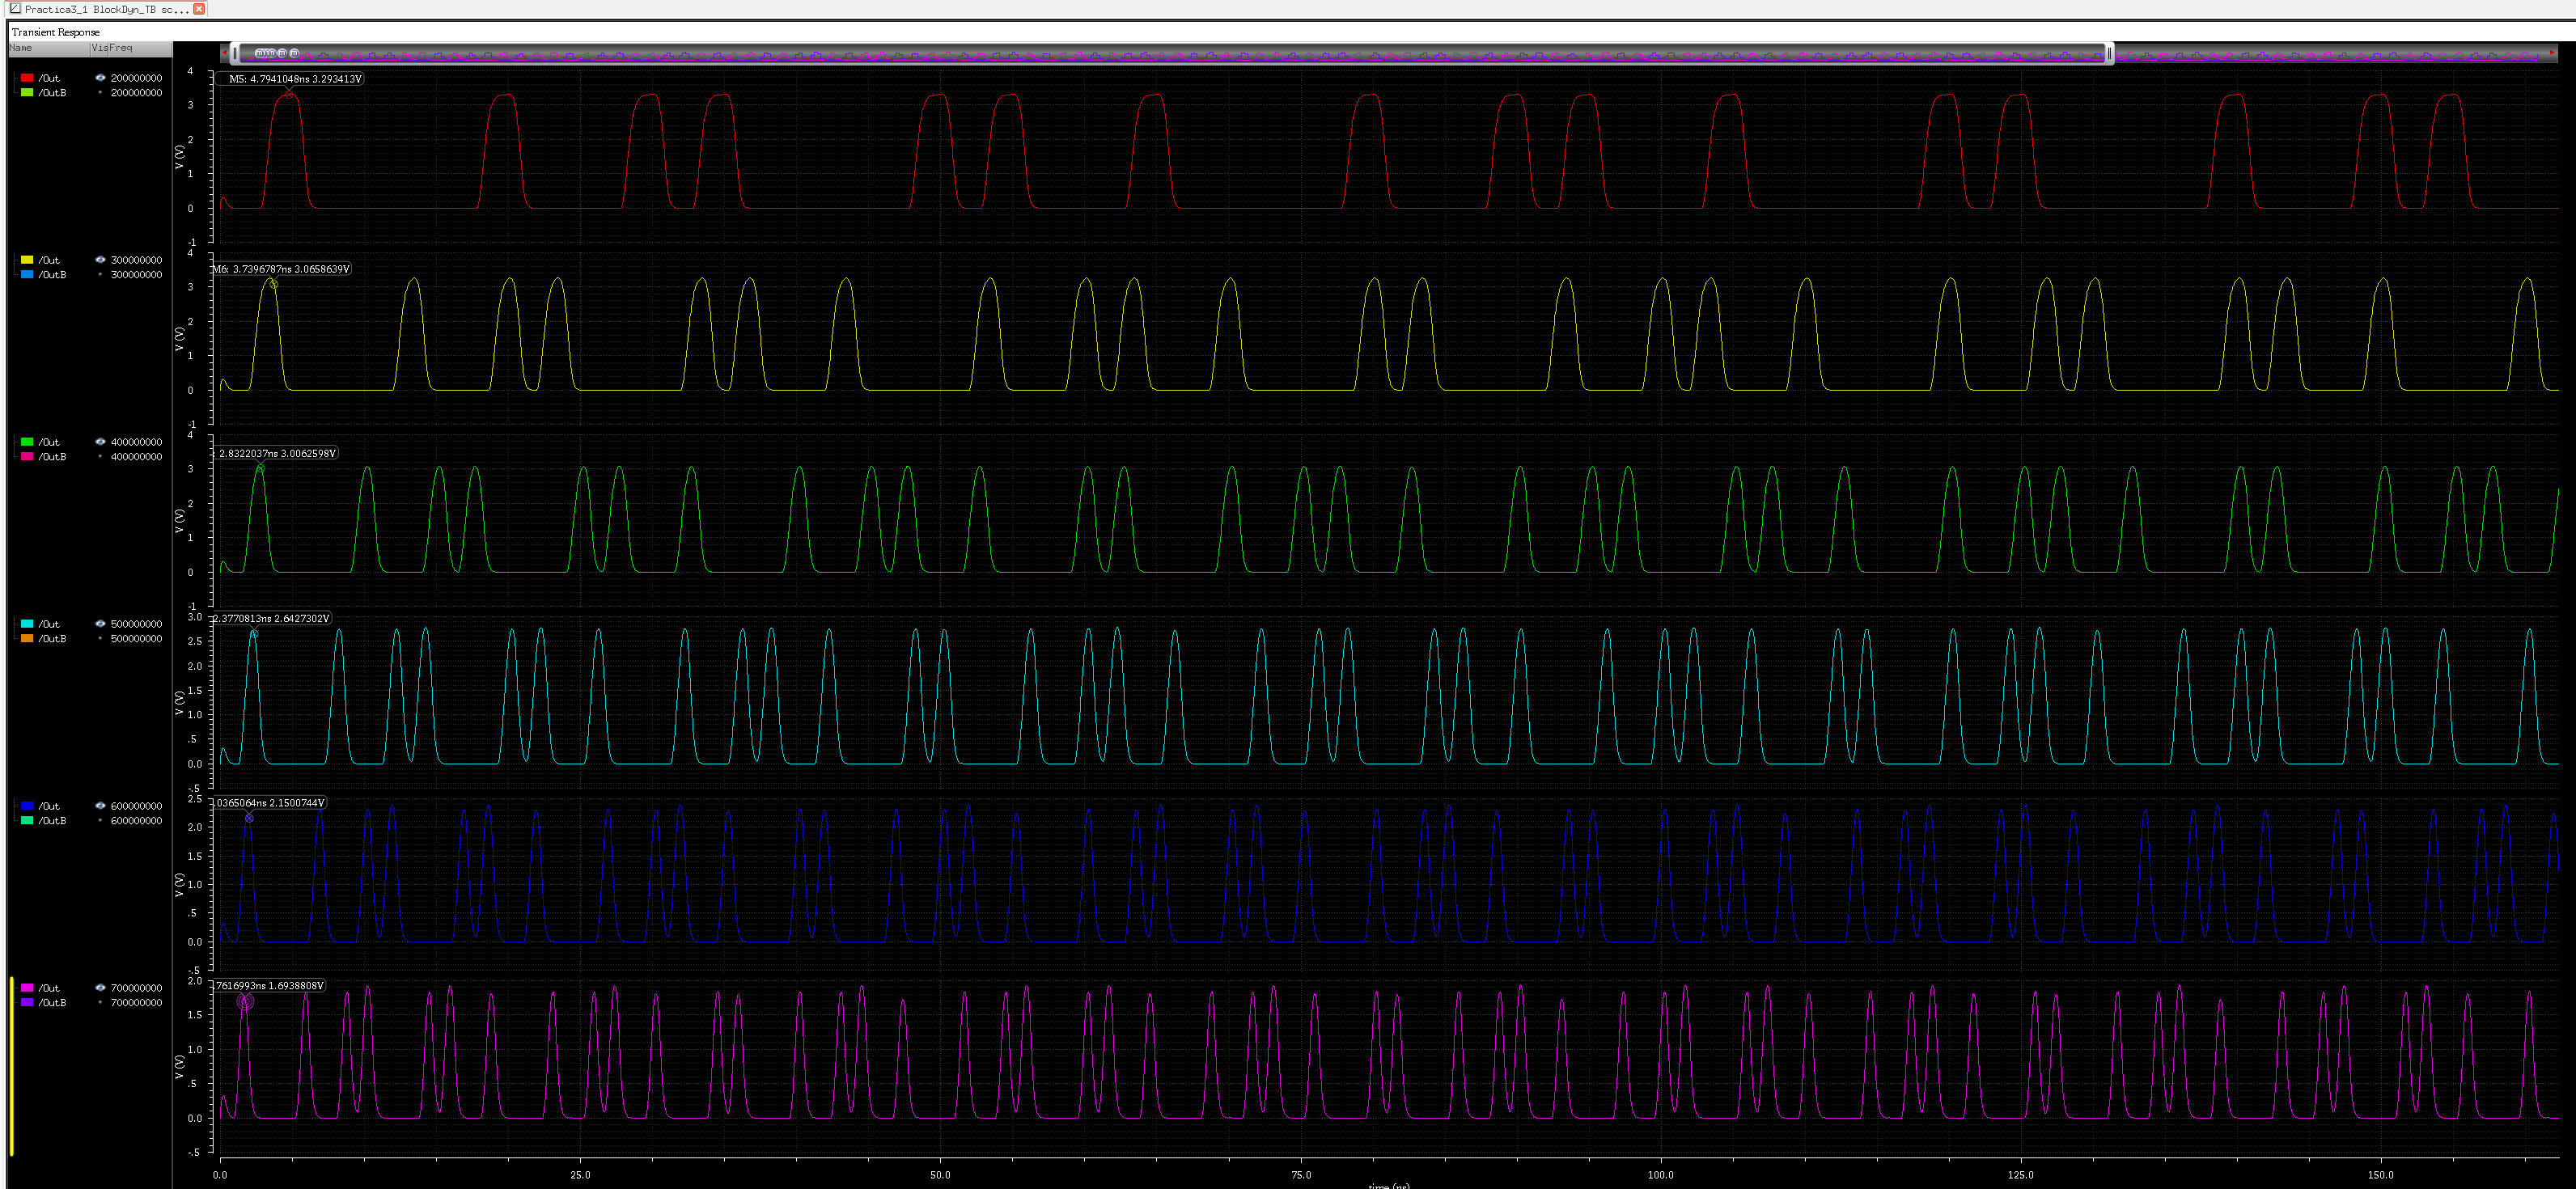
\includegraphics[width=1.1\textwidth]{figures/ParamFreqGraphNOVALIDO.PNG}
\caption{Gráfica del análisis paramétrico 200-700MHz}
\label{fig:GraphFreq1}
\end {center}
\end{figure} 
\vspace{-1cm}
\begin{figure}[H]%[!ht]
\begin {center}
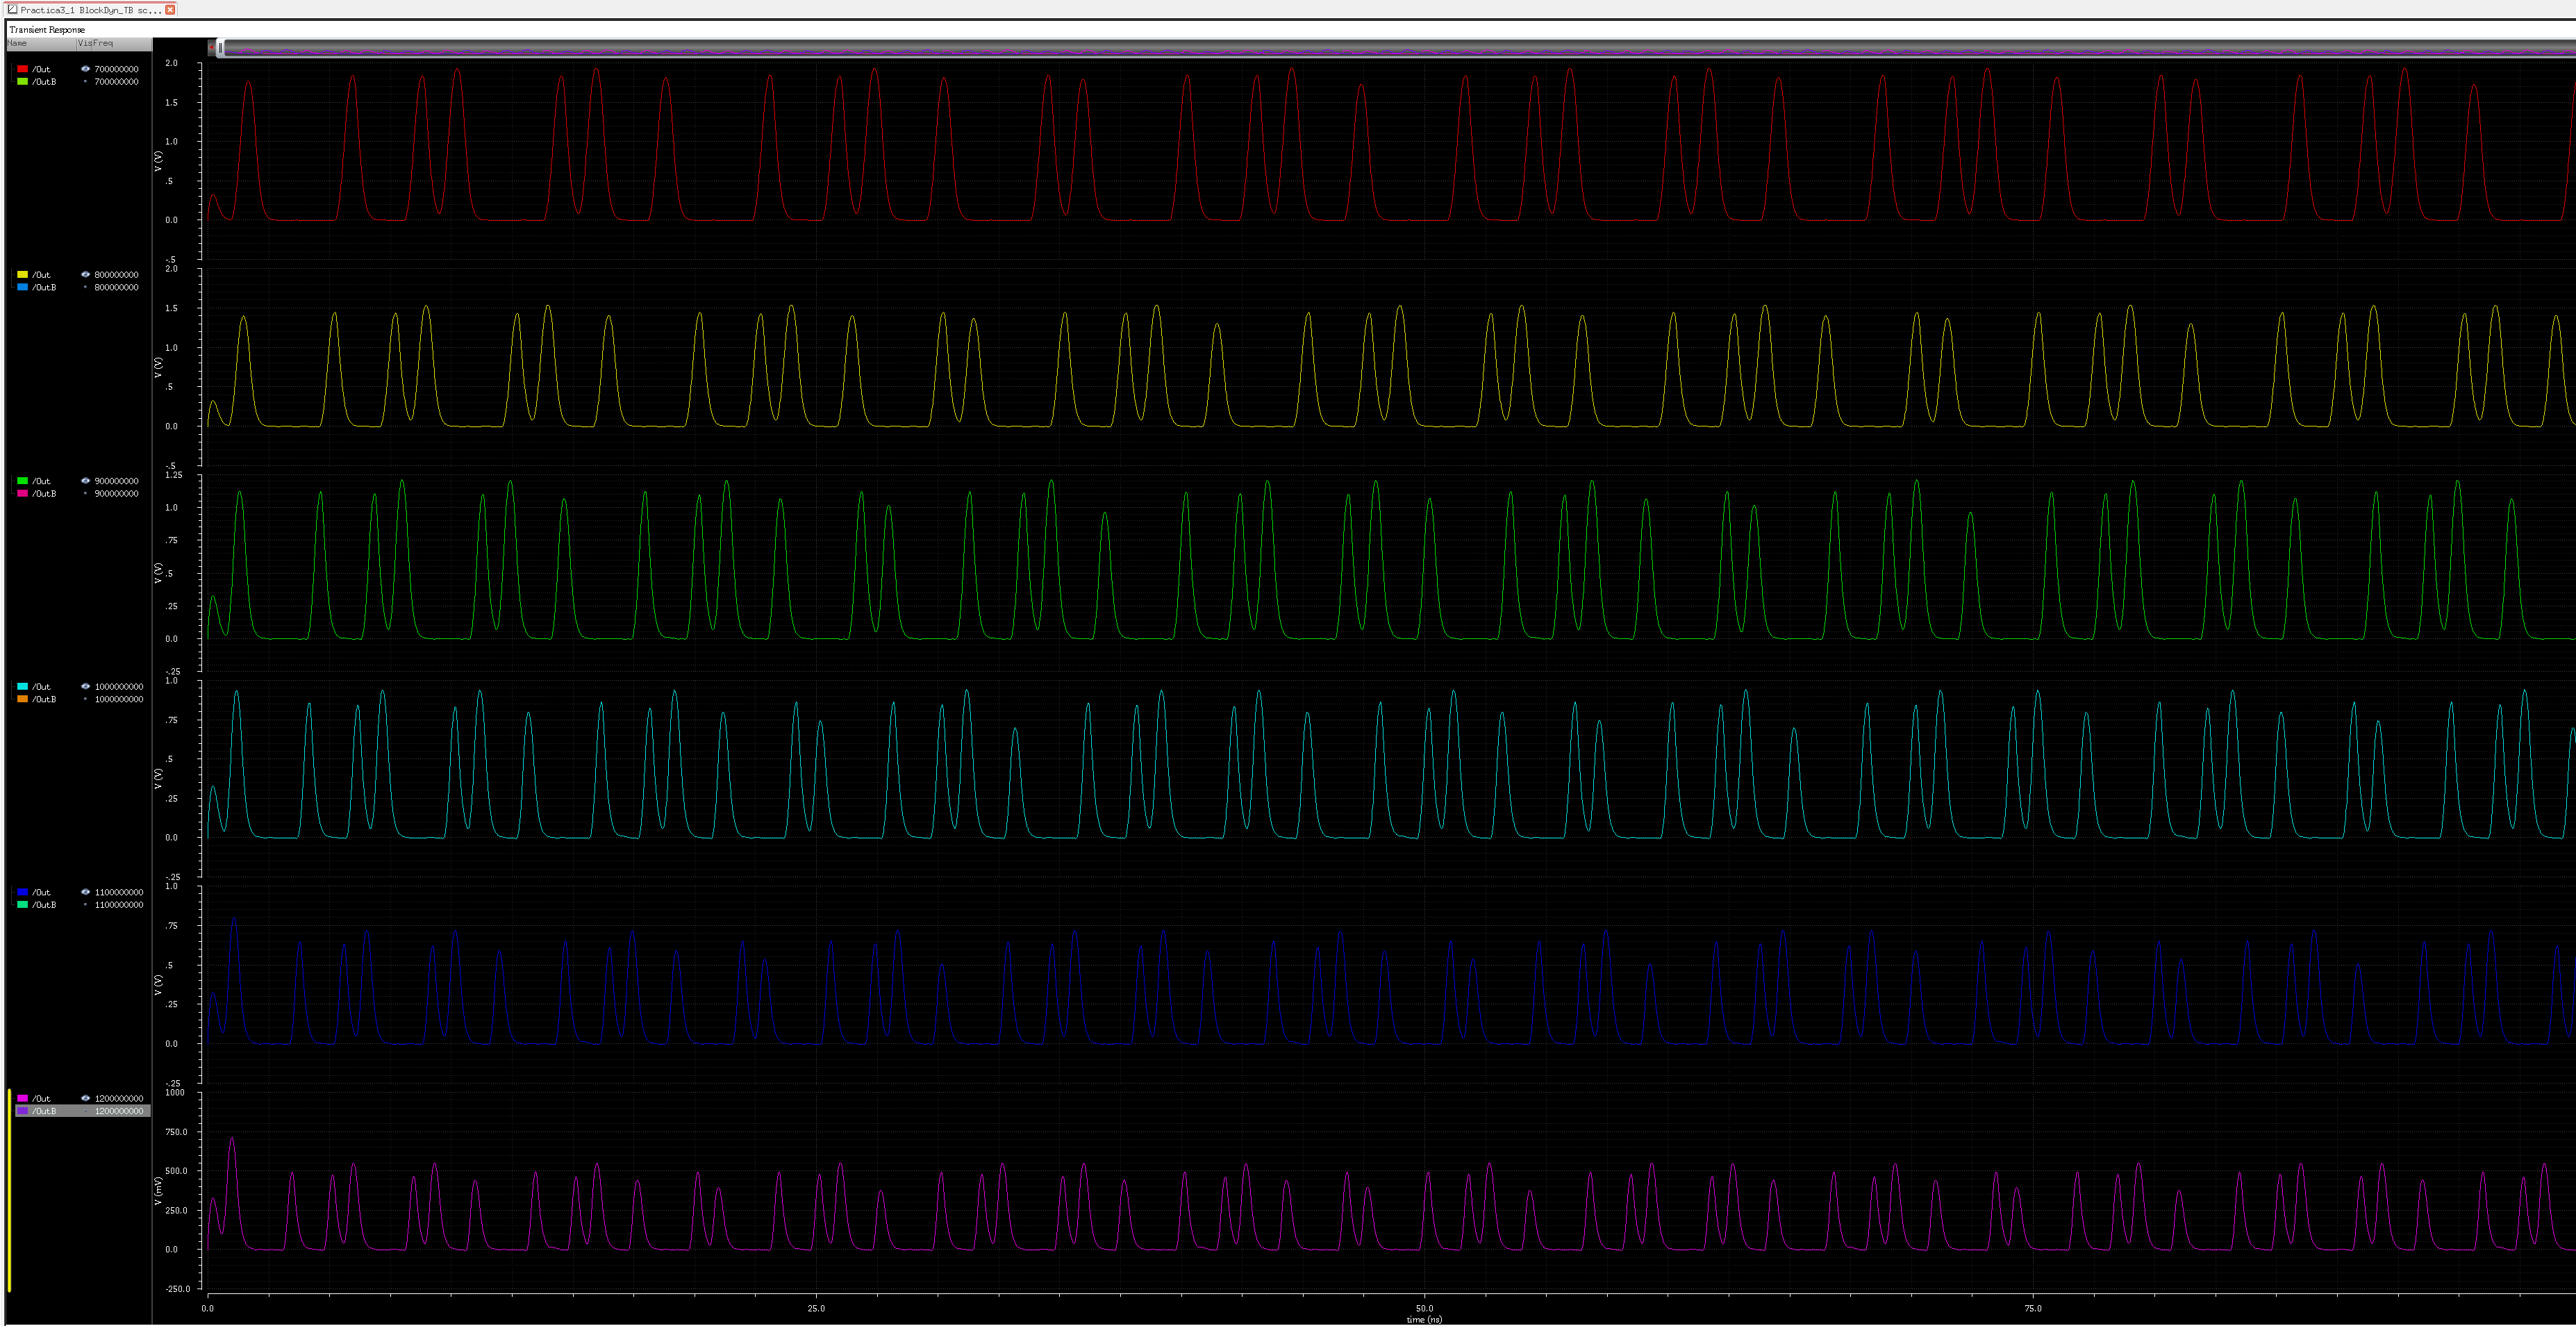
\includegraphics[width=1.1\textwidth]{figures/ParamFreqGraph2.PNG}
\caption{Gráfica del análisis paramétrico 700-1200MHz}
\label{fig:GraphFreq2}
\end {center}
\end{figure} 
Sólamente se muestra la salida Out para mayor claridad. Se puede observar que a medida que aumenta la frecuencia, el nivel de la salida se va reduciendo. Esto se debe a que como cada vez se le da menos tiempo a la evaluación, el nivel de la salida no le da tiempo a subir a un 1 cuando tiene que hacerlo desde el nivel bajo que supone la precarga en este caso. Alrededor de los 700MHz la señal ya llega sólo a la mitad de $V_{DD}$.

\newpage Pero, ¿qué pasaría si se realizara la simulación con un reloj asimétrico dedicándole más tiempo a la precarga o a la evaluación? Bien, estos fueron los resultados:
\begin{figure}[H]%[!ht]
\hspace{-10mm}
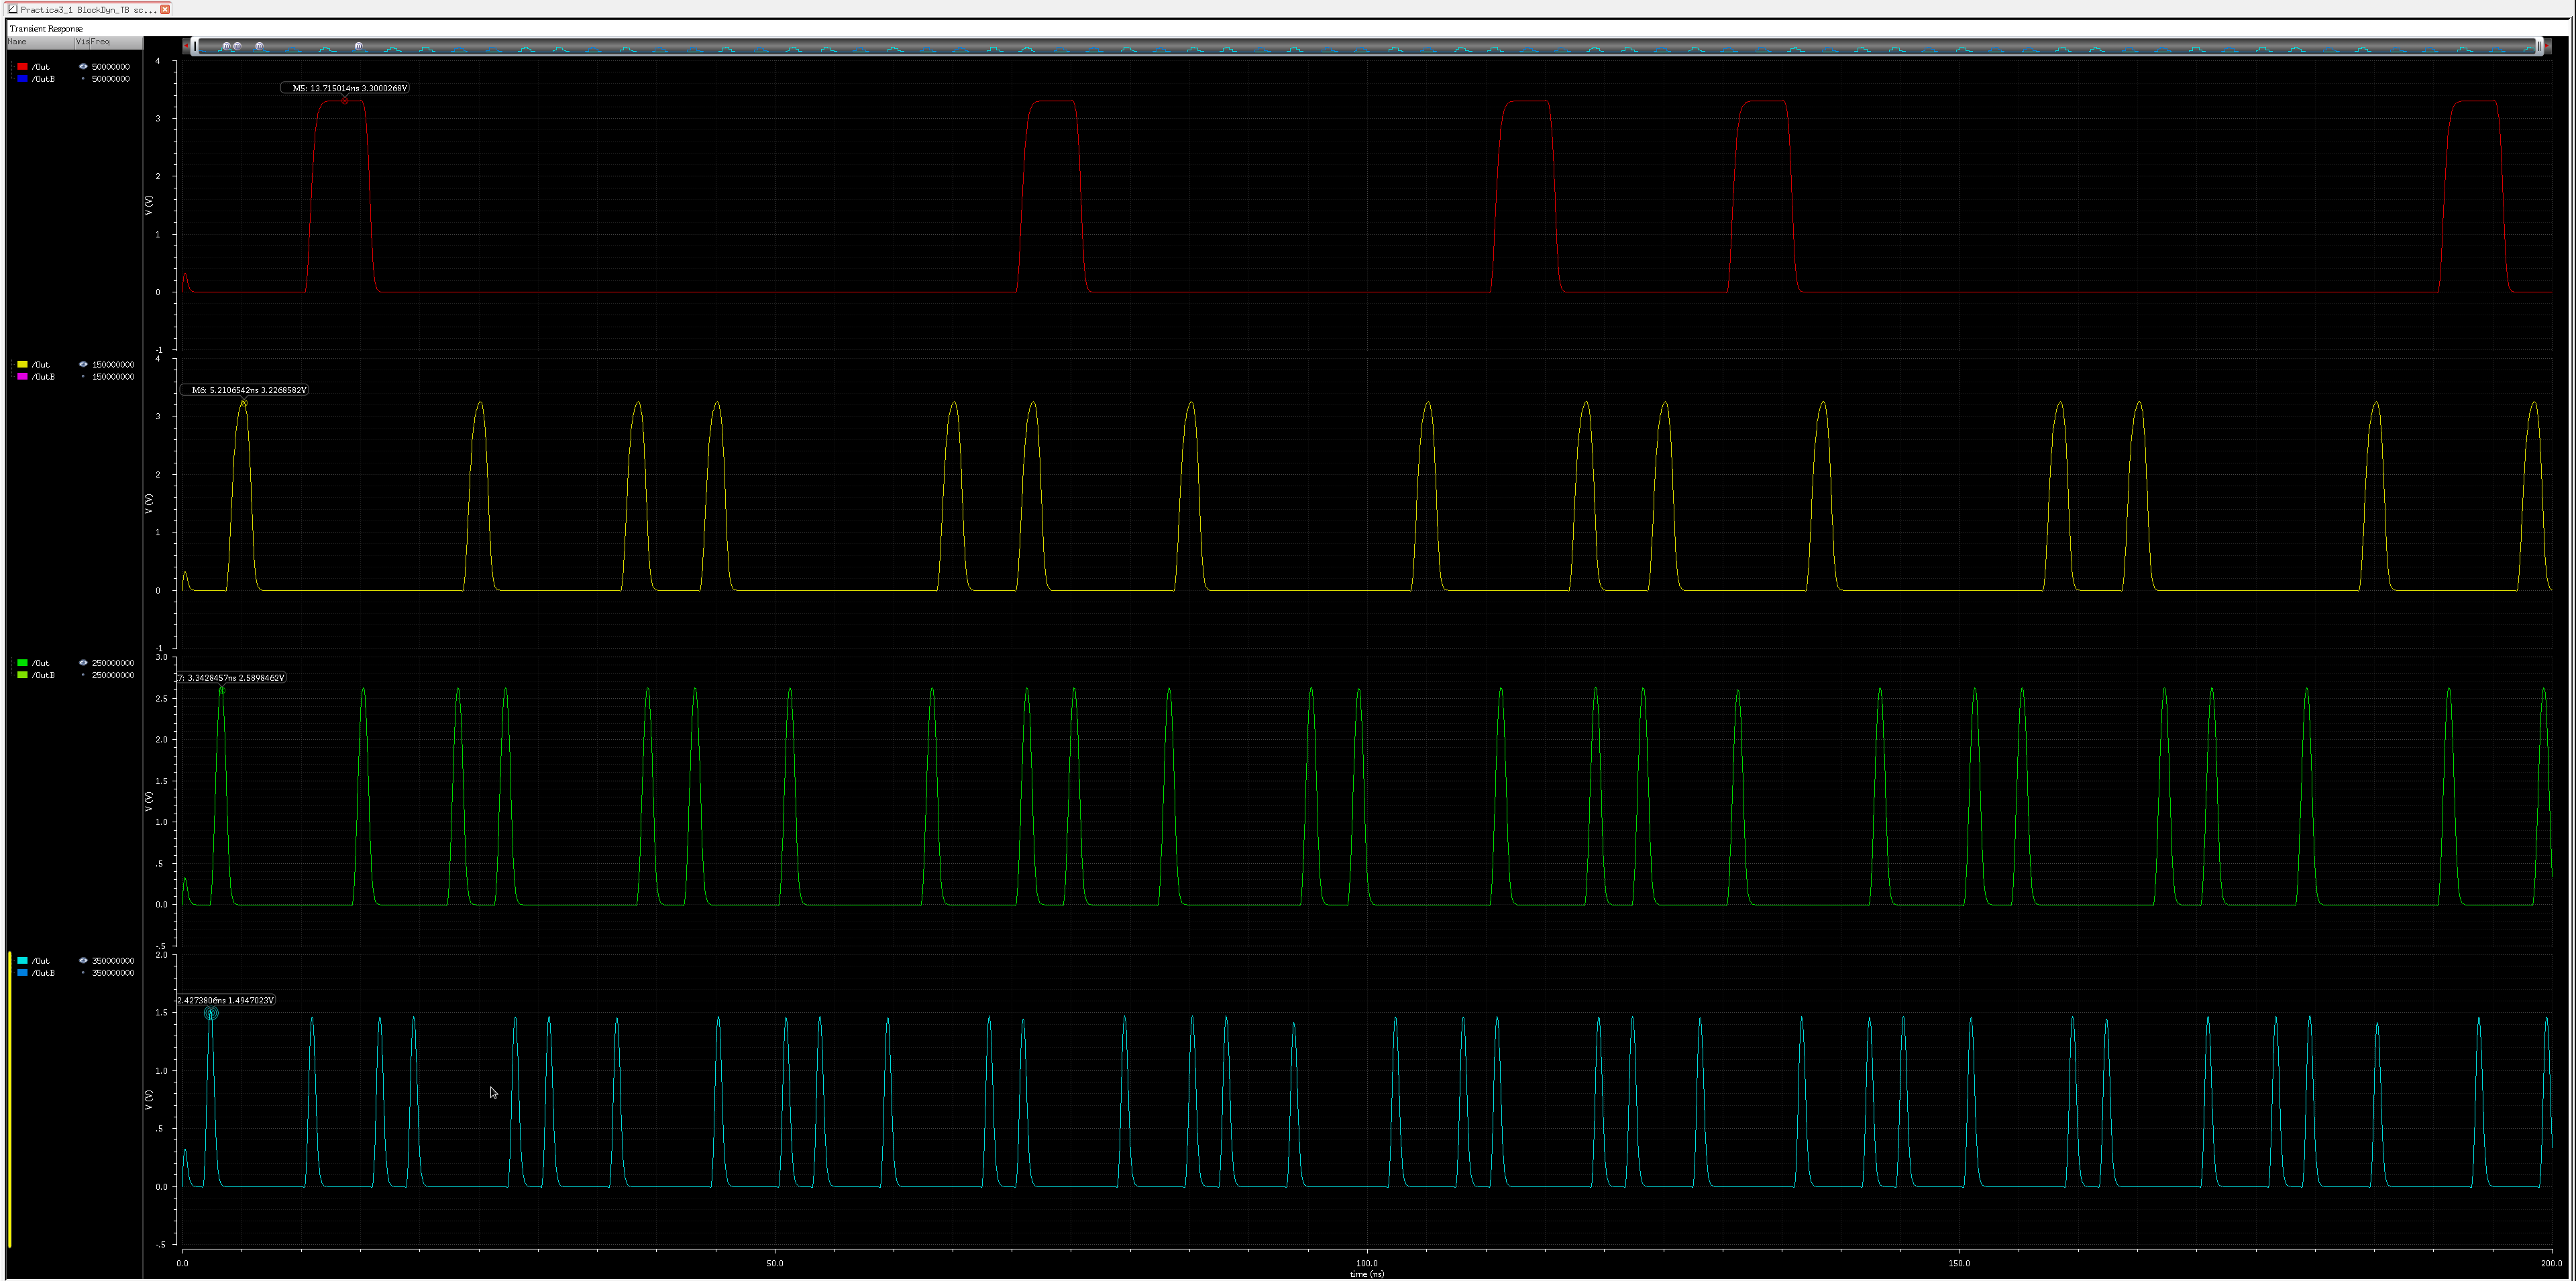
\includegraphics[width=1.2\textwidth]{figures/AsimMuchPreload.png}
\caption{Gráfica del análisis paramétrico 50-350MHz con un 75\% del reloj dedicado a la precarga}
\label{fig:FreqAsimPreload}
\end{figure}
\vspace{-8mm}
\begin{figure}[H]%[!ht]
\hspace{-10mm}
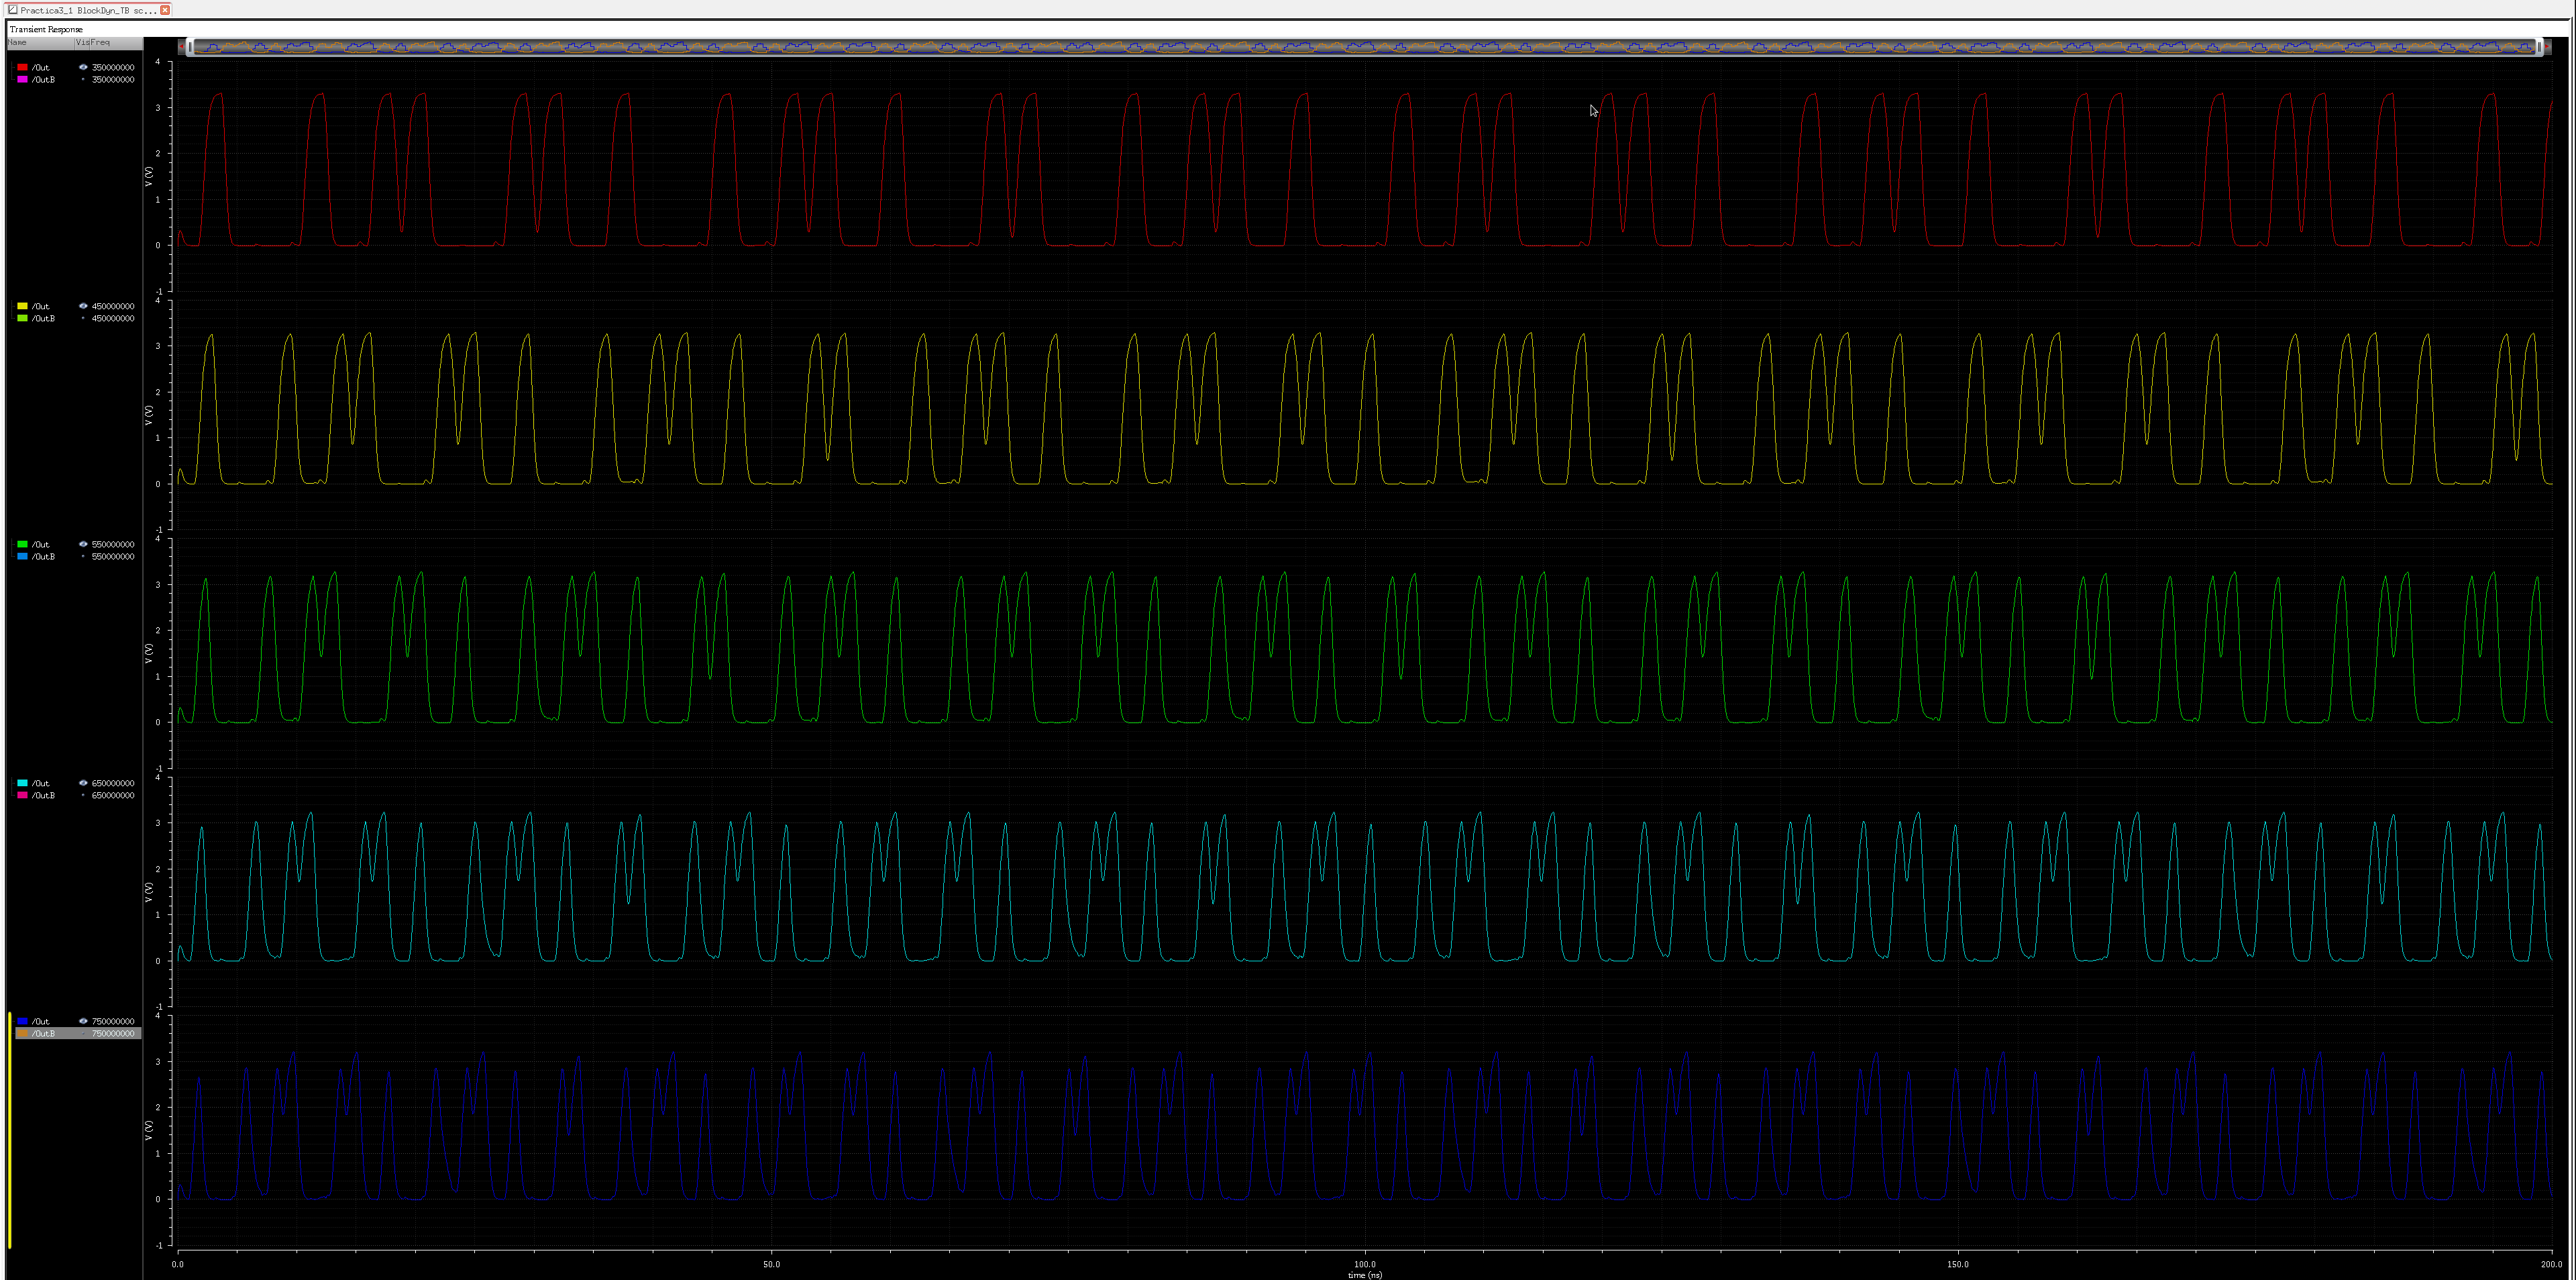
\includegraphics[width=1.2\textwidth]{figures/AsimMuchEval.png}
\caption{Gráfica del análisis paramétrico 350-750MHz con un 75\% del reloj dedicado a la evaluación}
\label{fig:FreqAsimEval}
\end{figure} 
Como se esperaba, la anchura de los pulsos aumenta cuando más porcentaje se le dedique a la evaluación. Además, el nivel de tensión es capaz de llegar los 3.3V a mayor frecuencia que si se le dedicara mayor porcentaje a la precarga. Sin embargo, hay solapamiento de niveles altos de señal a altas frecuencias en la figura \ref{fig:FreqAsimEval} debido a que la precarga dura demasiado poco como para ponerse la salida nivel bajo.
\subsection{Análisis paramétrico con la anchura $W_E$}
Como último paso en esta sección, se simularon para 500MHz de frecuencia, una simulación paramétrica sobre $W_E$, empleando el state anterior y con la siguiente configuración en \textit{Tools->Parametric Analysis}:
\begin{figure}[h]%[!ht]
\begin{center}
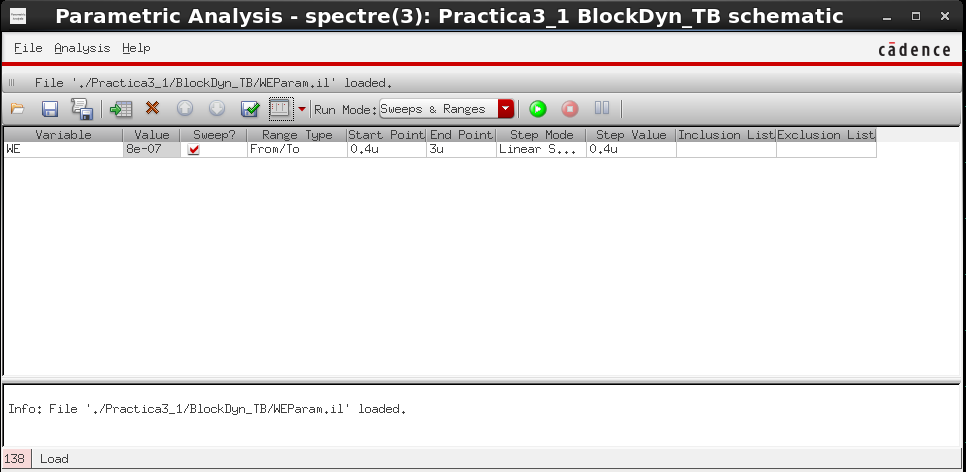
\includegraphics[width=0.8\textwidth]{figures/WEParamConfig.PNG}
\caption{Configuración del análisis paramétrico de $W_E$}
\label{fig:WEConfig}
\end{center}
\end{figure} \newline
Al correr la simulación, se obtuvo esta representación:
\begin{figure}[h]%[!ht]
\hspace{-10mm}
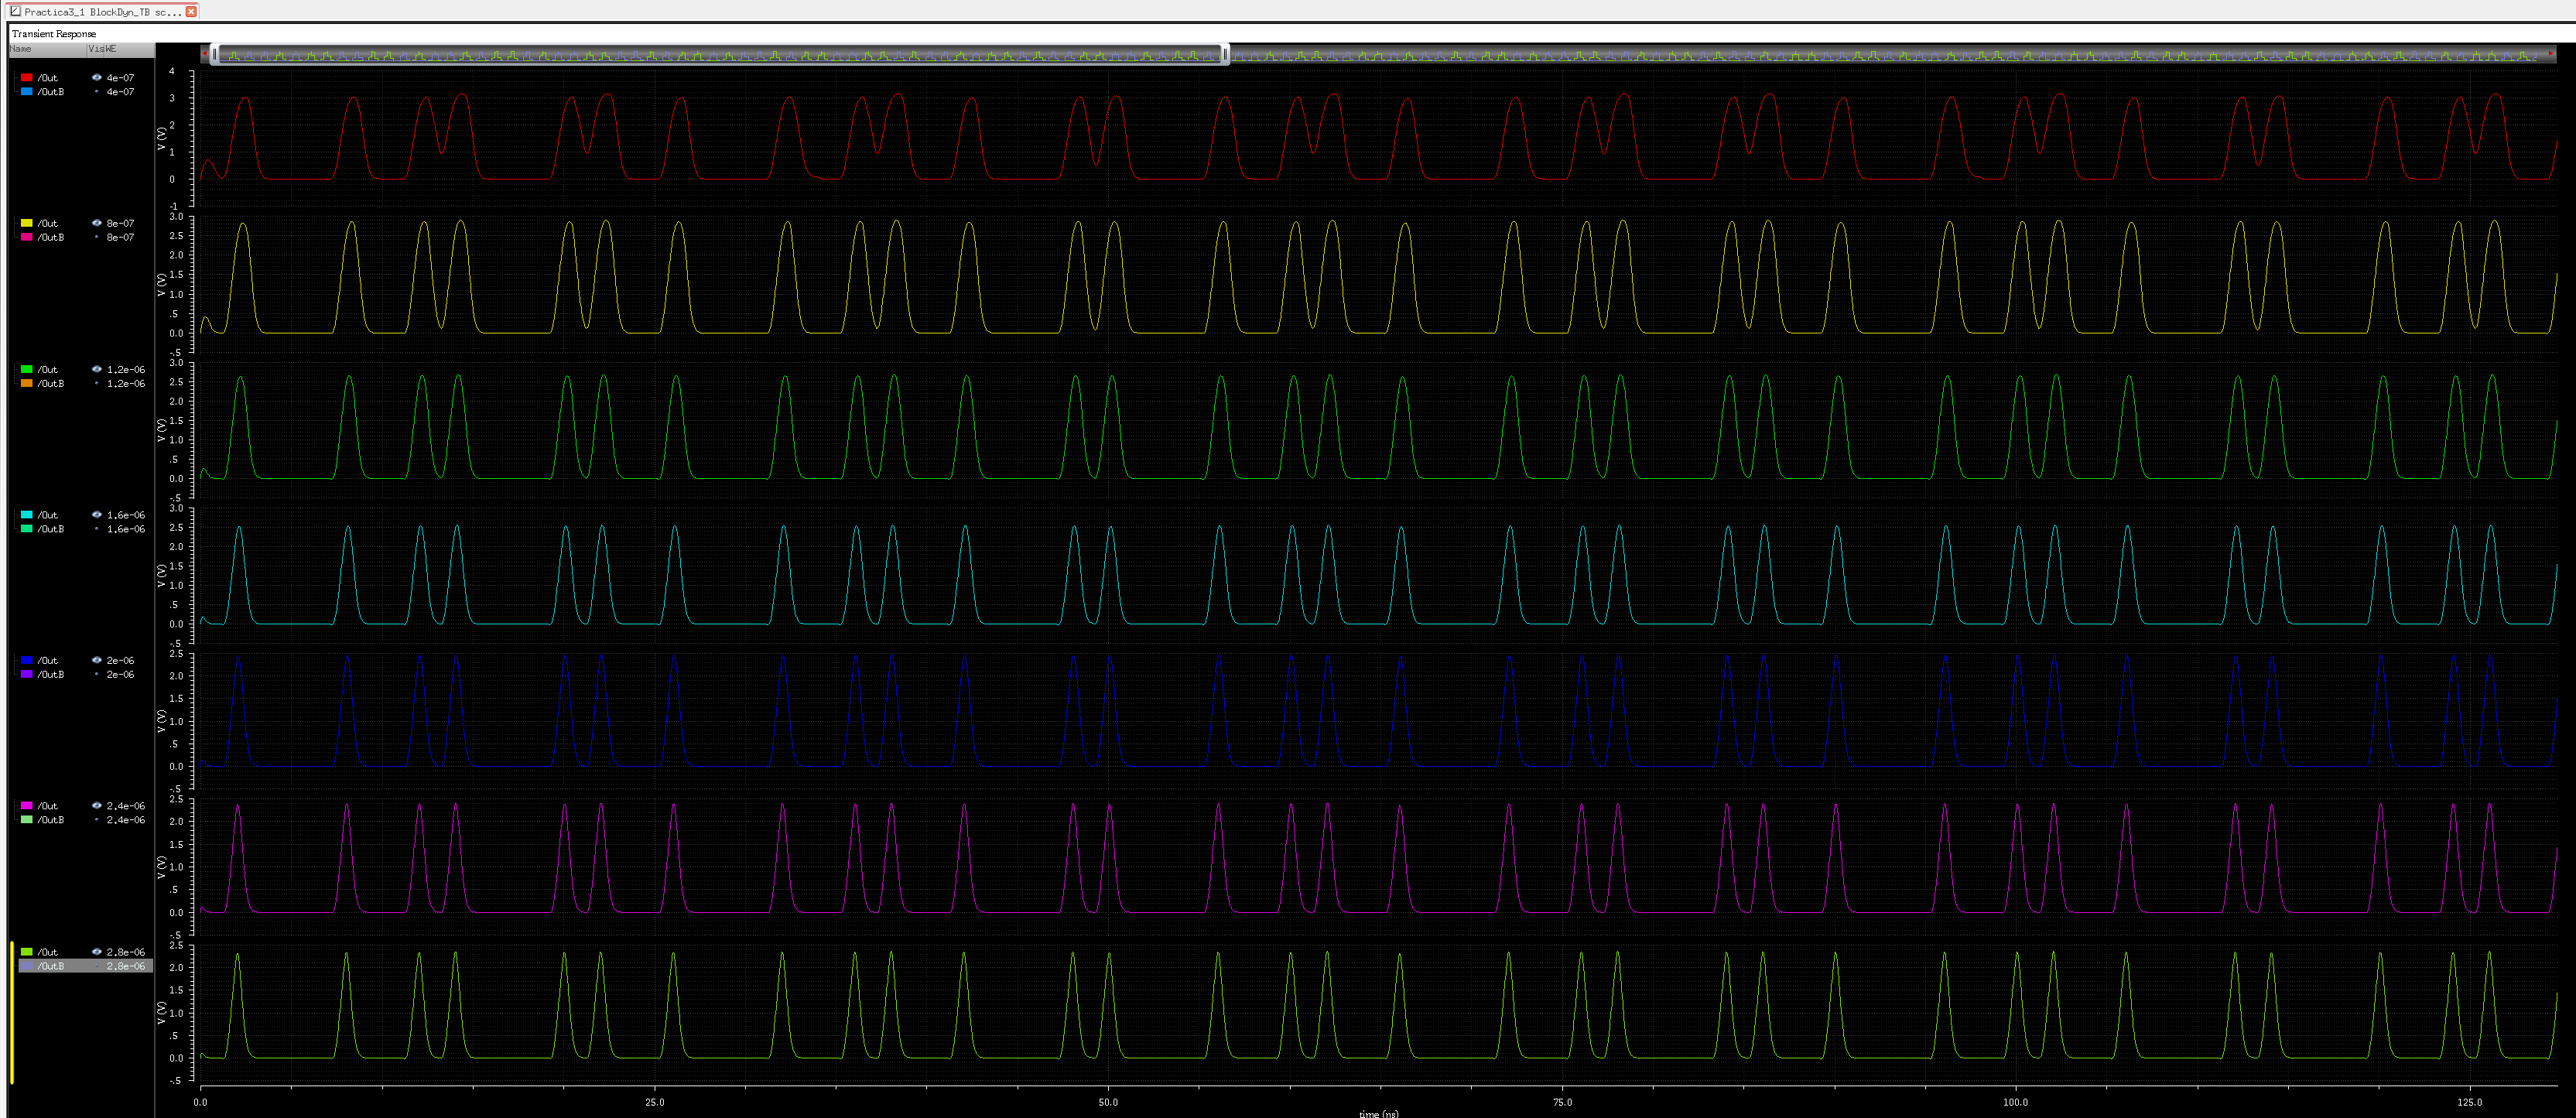
\includegraphics[width=1.2\textwidth]{figures/WEGraph.PNG}
\caption{Gráfica del análisis paramétrico 0.4-3$\mu m$}
\label{fig:WEGraph}
\end{figure} \newline
No se debe aumentar mucho el parámetro $W_E$ ya que ello supone un aumento en el espacio ocupado y mayor carga capacitiva en la línea del reloj, lo que haría que el nivel de la señal se redujera como se ve en los valores más altos de $W_E$ del análisis paramétrico. Por ahora, si se compara con nuestra figura de referencia \ref{fig:GraphState1}, vemos que Out tiene la misma secuencia de valores por lo que la evaluación de momento, está bien con la salvedad del nivel de tensión a la salida ya comentado anteriormente.
\newpage Al igual que con el análisis en frecuencia, se cambió el reloj simétrico por uno asimétrico y, volviéndose a ejecutar la simulación, estos fueron los resultados:
\begin{figure}[H]%[!ht]
\hspace{-10mm}
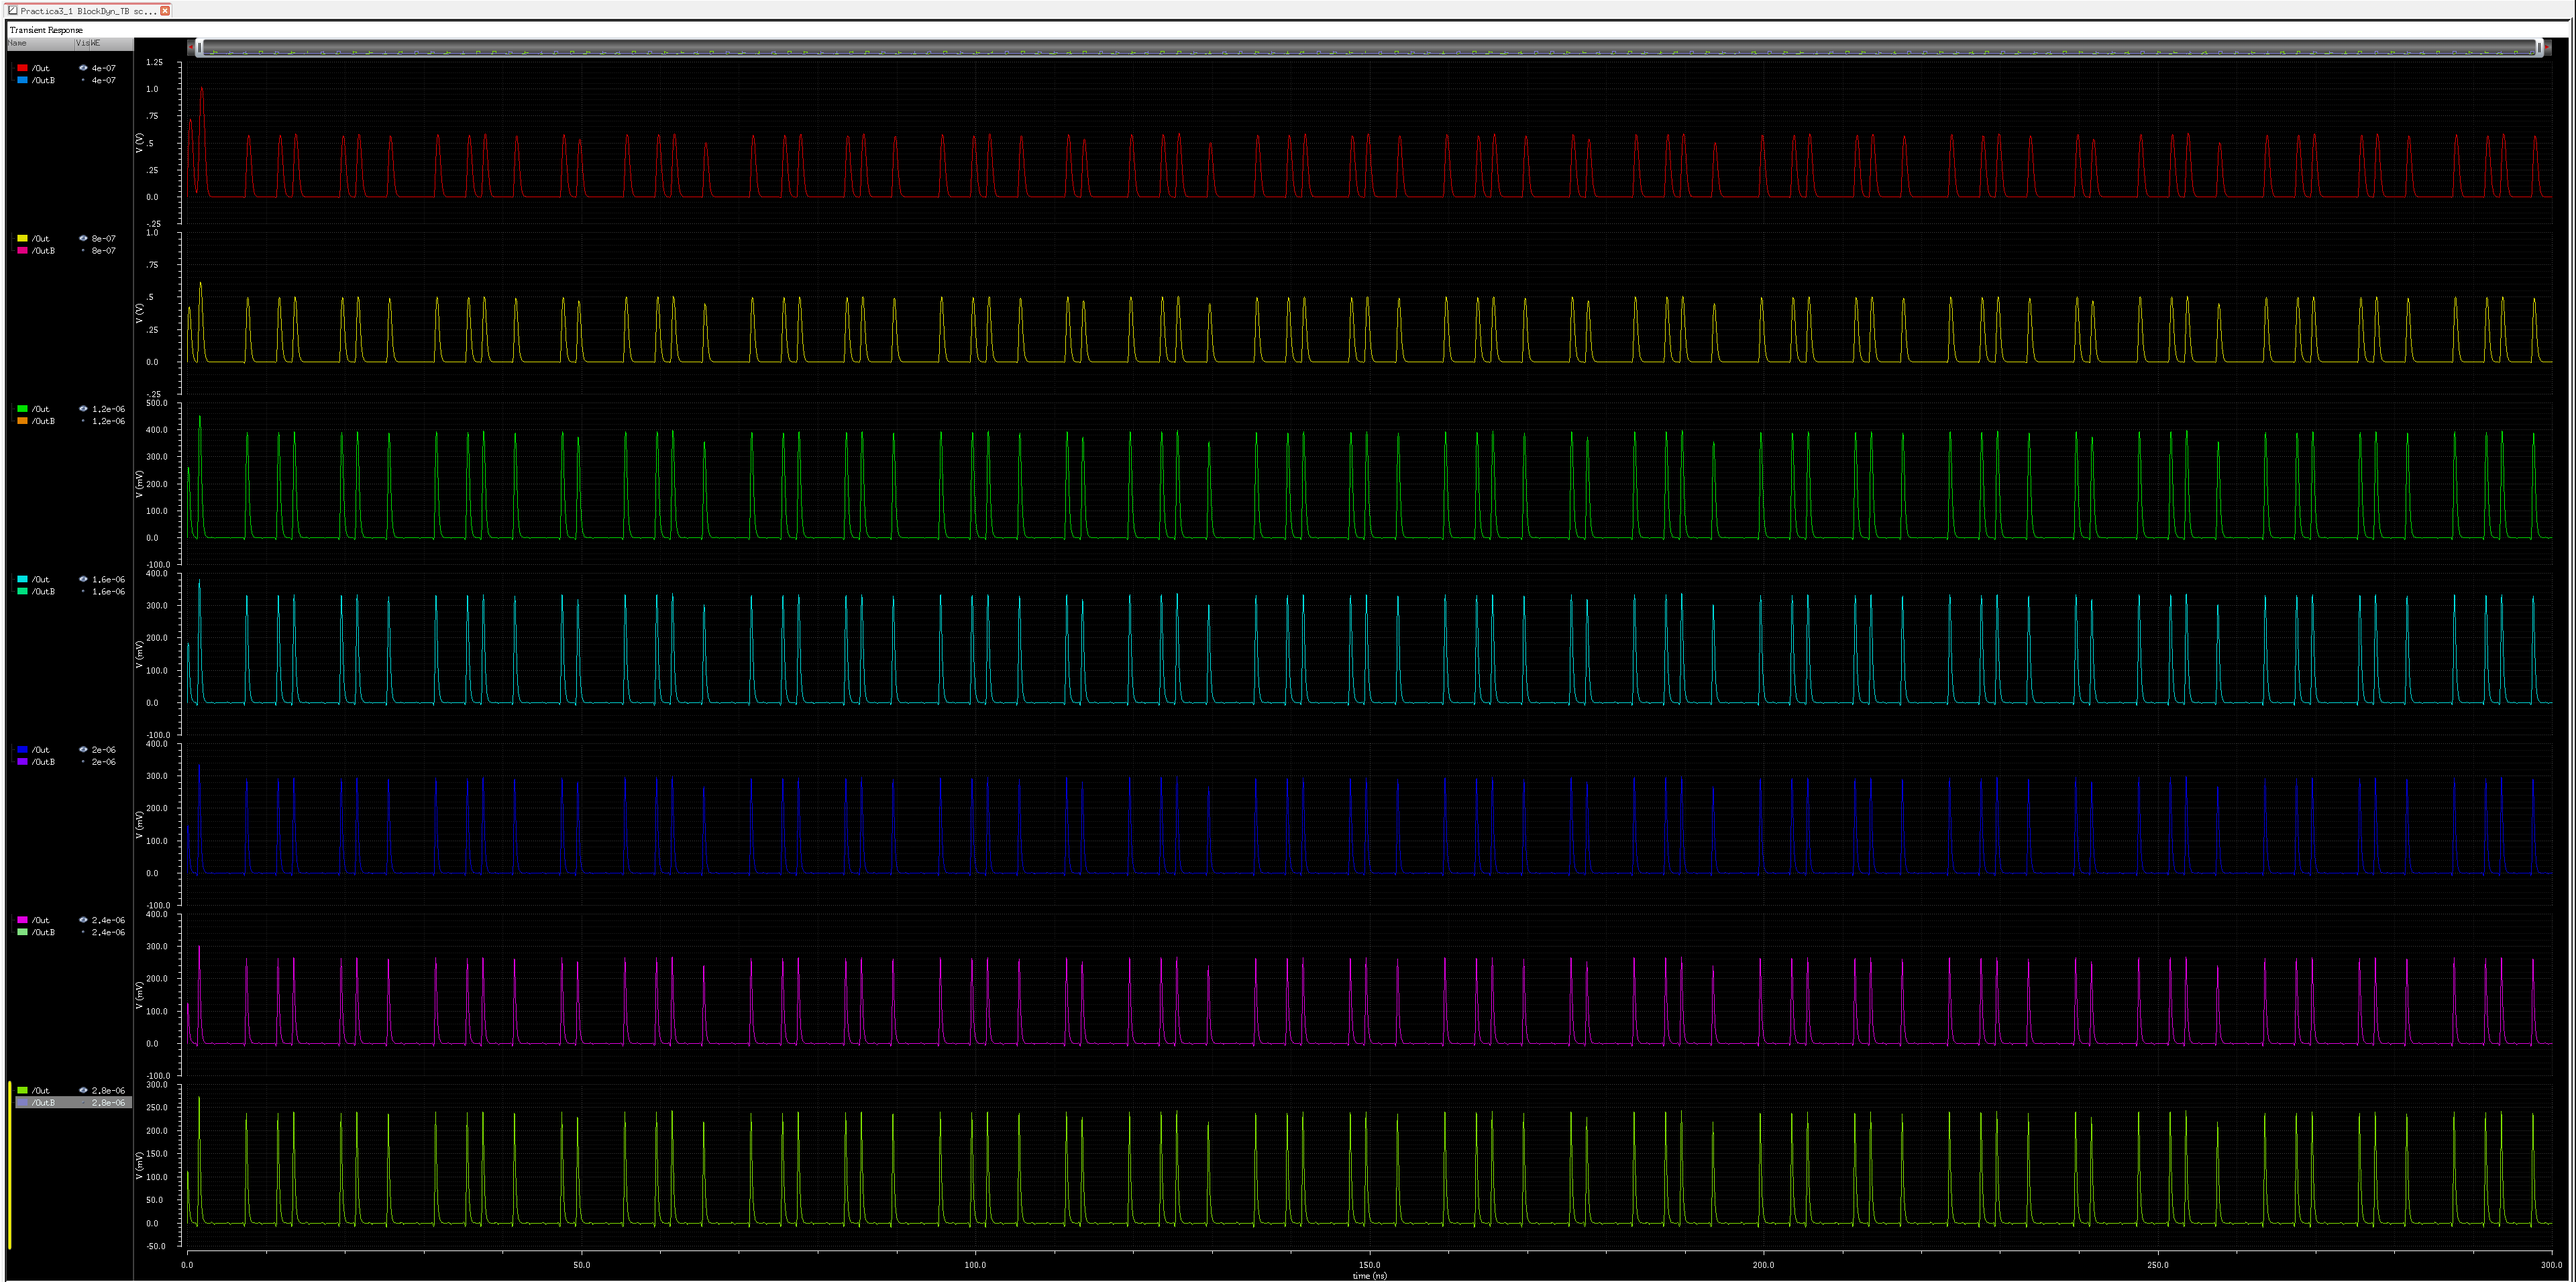
\includegraphics[width=1.2\textwidth]{figures/WEAsimMuchPreload.png}
\caption{Gráfica del análisis paramétrico 0.4-3$\mu m$ con un 75\% del reloj dedicado a la precarga}
\label{fig:WEAsimPreload}
\end{figure}
\vspace{-8mm}
\begin{figure}[H]%[!ht]
\hspace{-10mm}
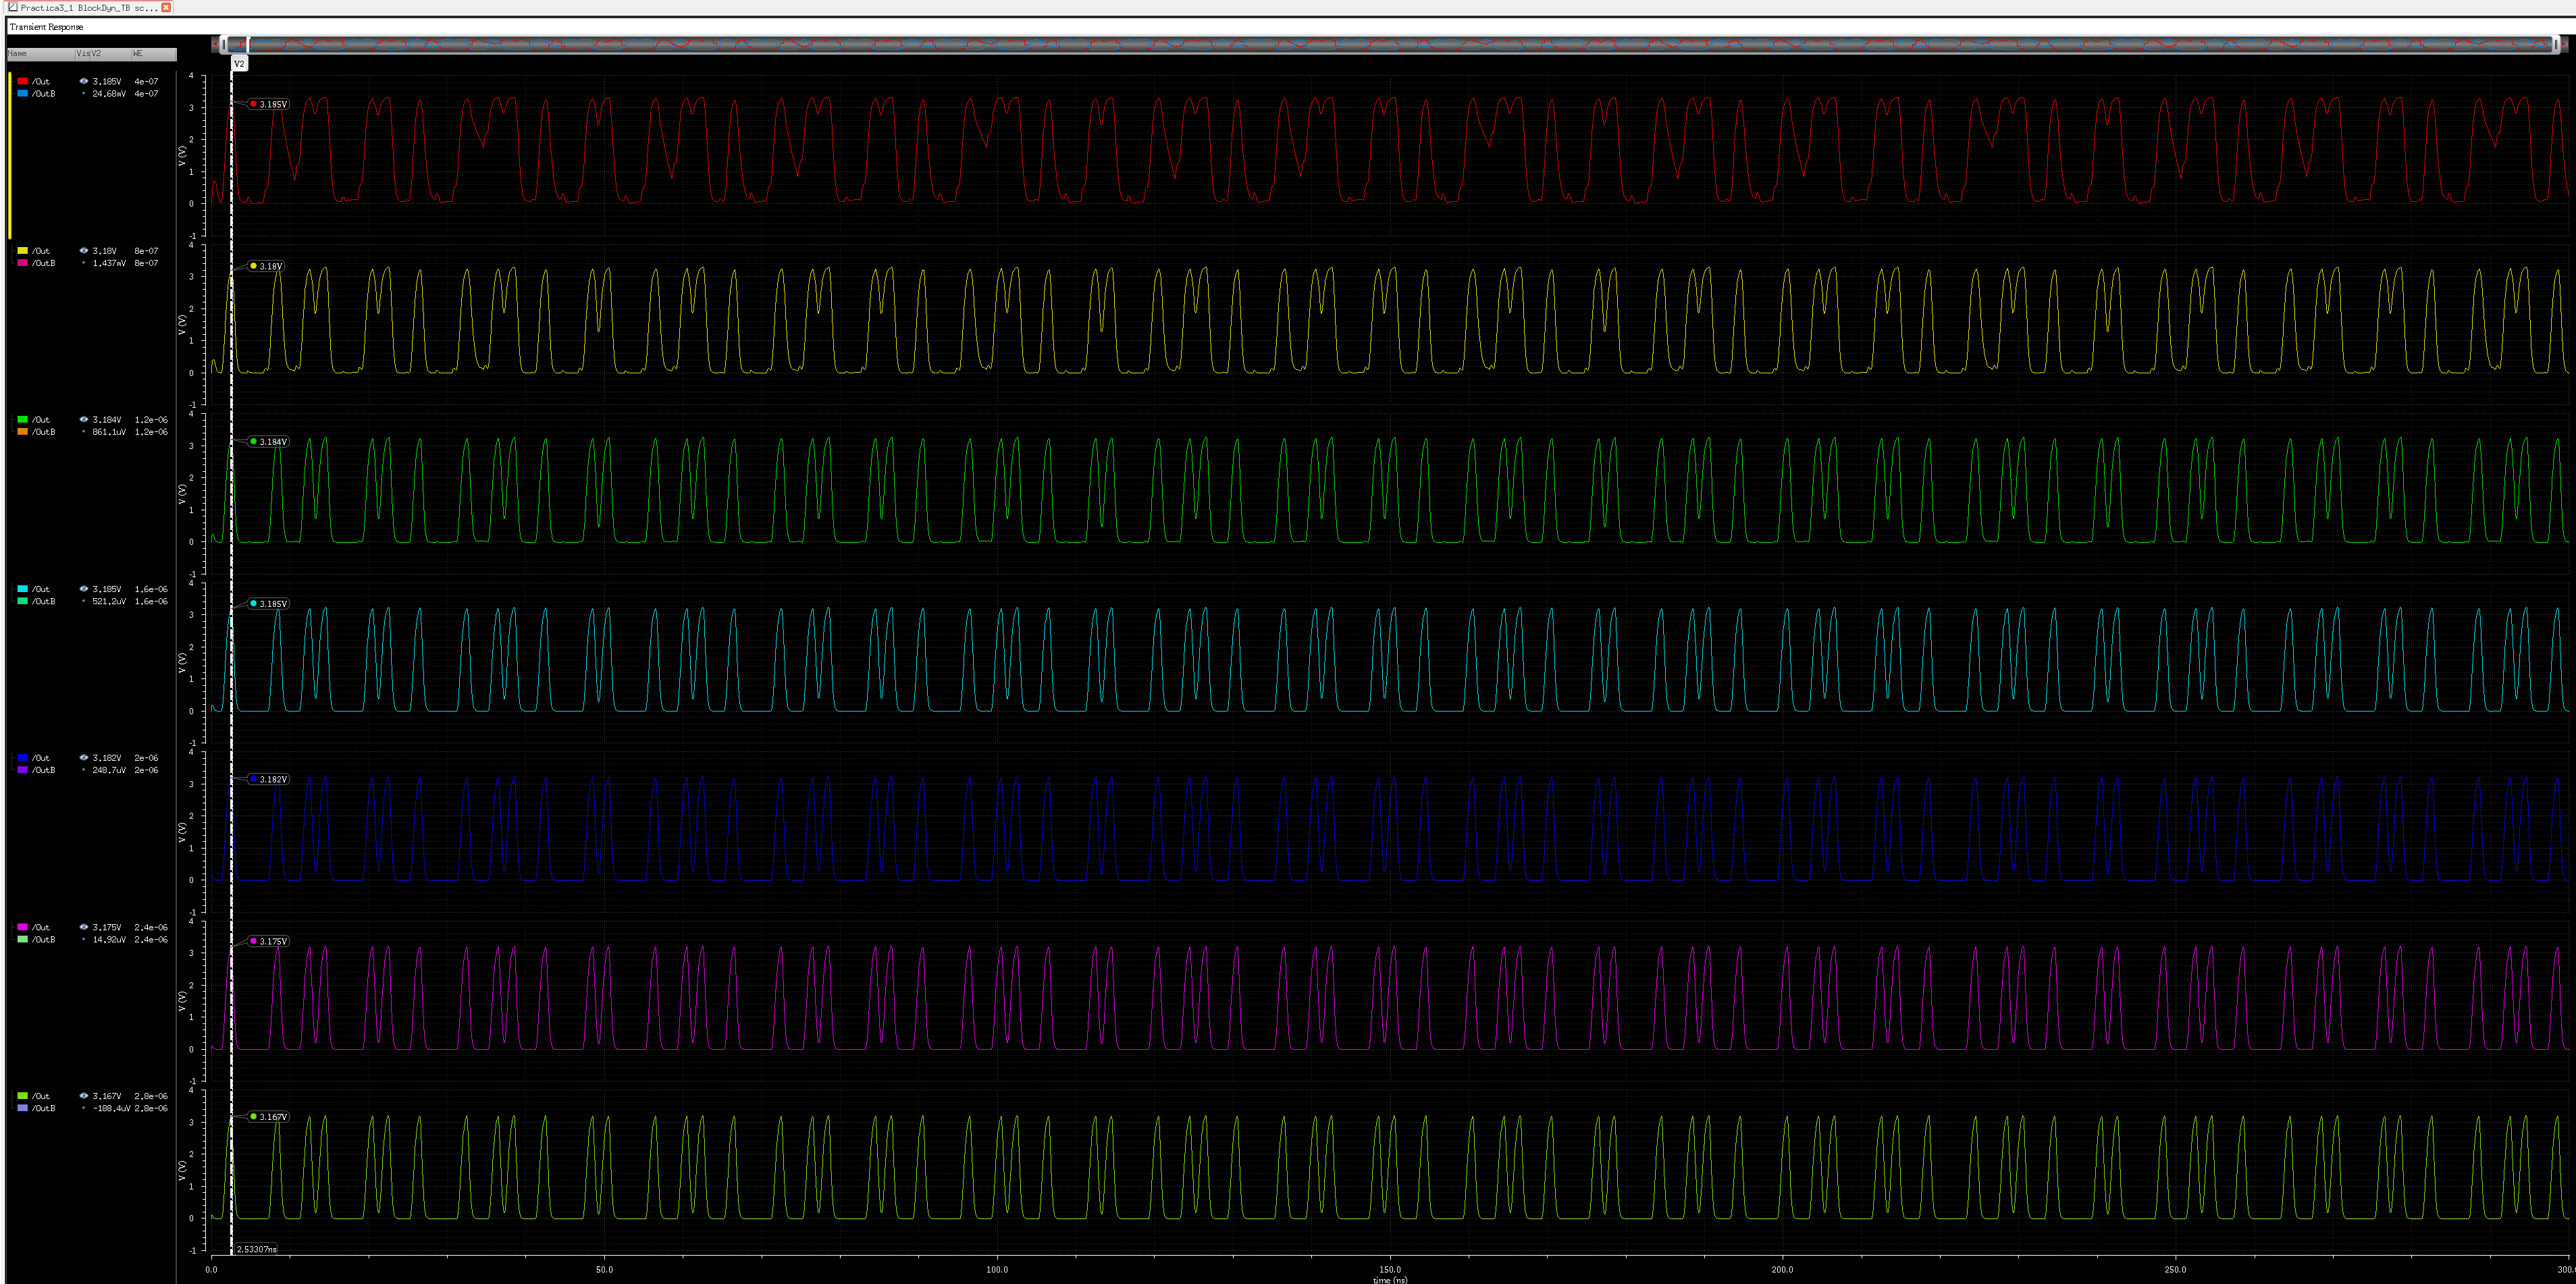
\includegraphics[width=1.2\textwidth]{figures/WEAsimMuchEval.png}
\caption{Gráfica del análisis paramétrico 0.4-3$\mu m$ con un 75\% del reloj dedicado a la evaluación}
\label{fig:WEAsimEval}
\end{figure} 
Si se le dedica demasiado tiempo a la evaluación, la anchura mínima $W_E$ que se debe coger aumenta. Esto se debe a que a mayor $W_E$, mejor evaluación (sin pasarnos mucho con este valor). En caso contrario, debido a que la precarga dura mucho, cuando se debe poner a 1 la salida, esta tiene demasiado poco tiempo para hacerlo y, por tanto no llega a los niveles de tensión requeridos. Habría que coger una $W_E$ más pequeña para disminuir la resistencia y la capacidad de los nMOS y conseguir así alcanzar el valor de tensión de nivel alto.
\restoregeometry

\chapter{Encadenado de etapas dinámicas}\label{ch:ch3label}
\section{Introducción}
El inconveniente de la lógica dinámica es que no se pueden encadenar en cascado las etapas como sí se podría hacer con la lógica estática, sino que debemos procurar una buena conexión para que funcione.
\section{Esquemático del circuito}
En este apartado se ha dibujado otro banco de pruebas esta vez con dos BlockDyn encadenados entre sí:
\begin{figure}[h]%[!ht]
\begin {center}
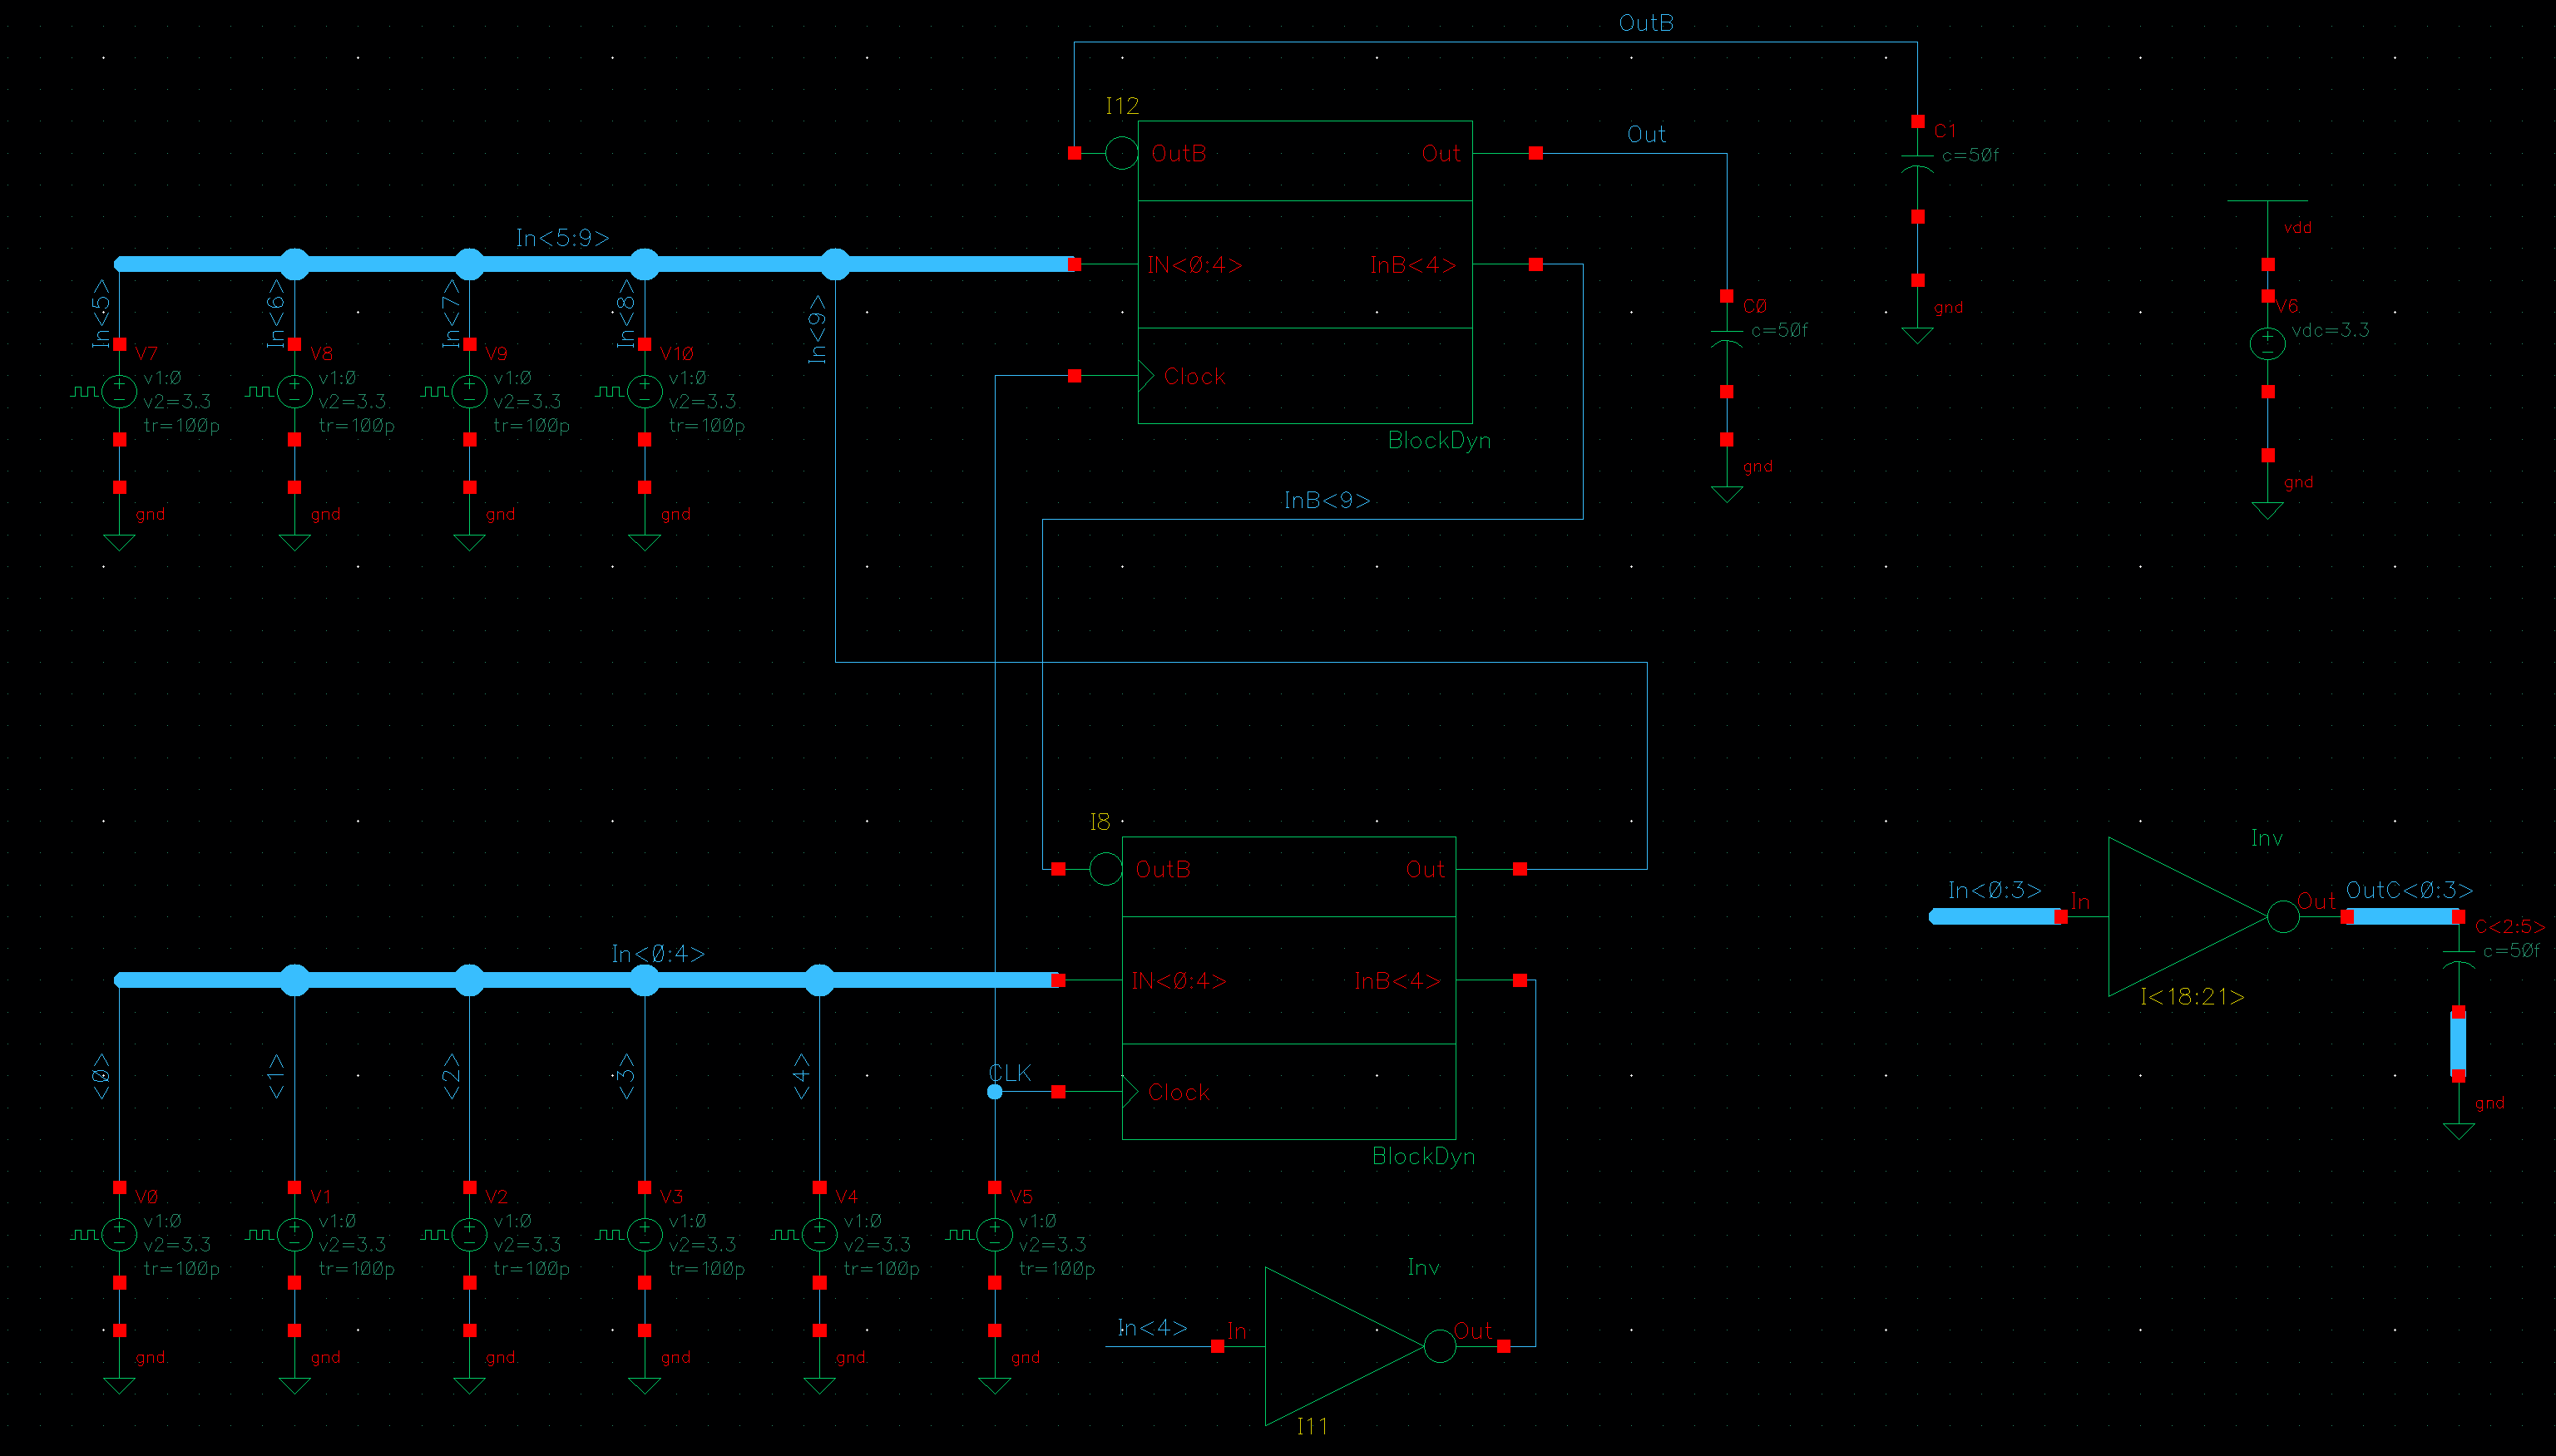
\includegraphics[width=1.1\textwidth]{figures/BlockDynEncTBSchem.PNG}
\caption{Banco de pruebas de 2 etapas BlockDyn correctamente encadenadas}
\label{fig:SchemTBEnc}
\end {center}
\end{figure} \newline
Apréciense la forma especial en la que se deben conectar los 2 bloques, siempre la salida del anterior al último bit de entrada de la siguiente, nunca a ningún otro. Se hará una simulación para ver qué pasa en caso de no cumplirse esta afirmación. \newgeometry{top=3cm, bottom=2cm}
\section{Análisis transitorio}
\par En primer lugar, se ha creado un estado nuevo con una frecuencia de 200MHz y un tiempo de simulación de 1.5u para ver todas las combinaciones posibles:
\begin{figure}[h]%[!ht]
\begin {center}
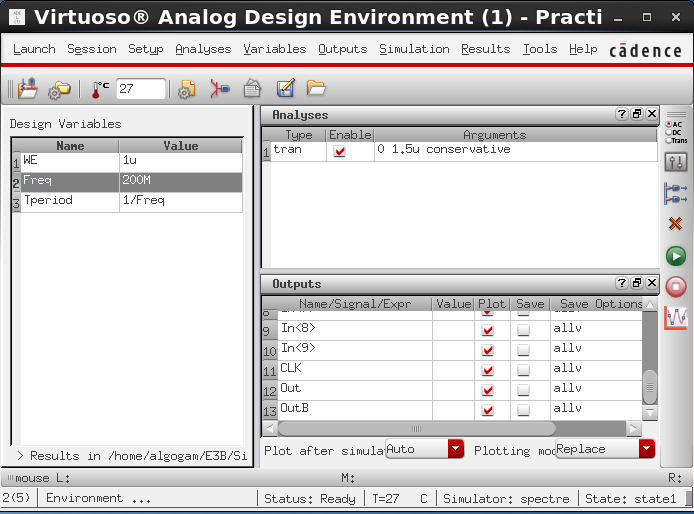
\includegraphics[width=0.7\textwidth]{figures/StateEncConfig.PNG}
\caption{Configuración del ADE para el banco de pruebas del encadenado}
\label{fig:ConfigTBEnc}
\end {center}
\end{figure} \newline
Sin embargo, en la captura que aquí se muestra, se ha hecho un zoom a los primeros 400ns para tener una mejor visión de las salidas, ya que estás aparecían demasiado estrechas si se tomaba una captura del tiempo de simulación completo:
\begin{figure}[H]%[!ht]
\begin {center}
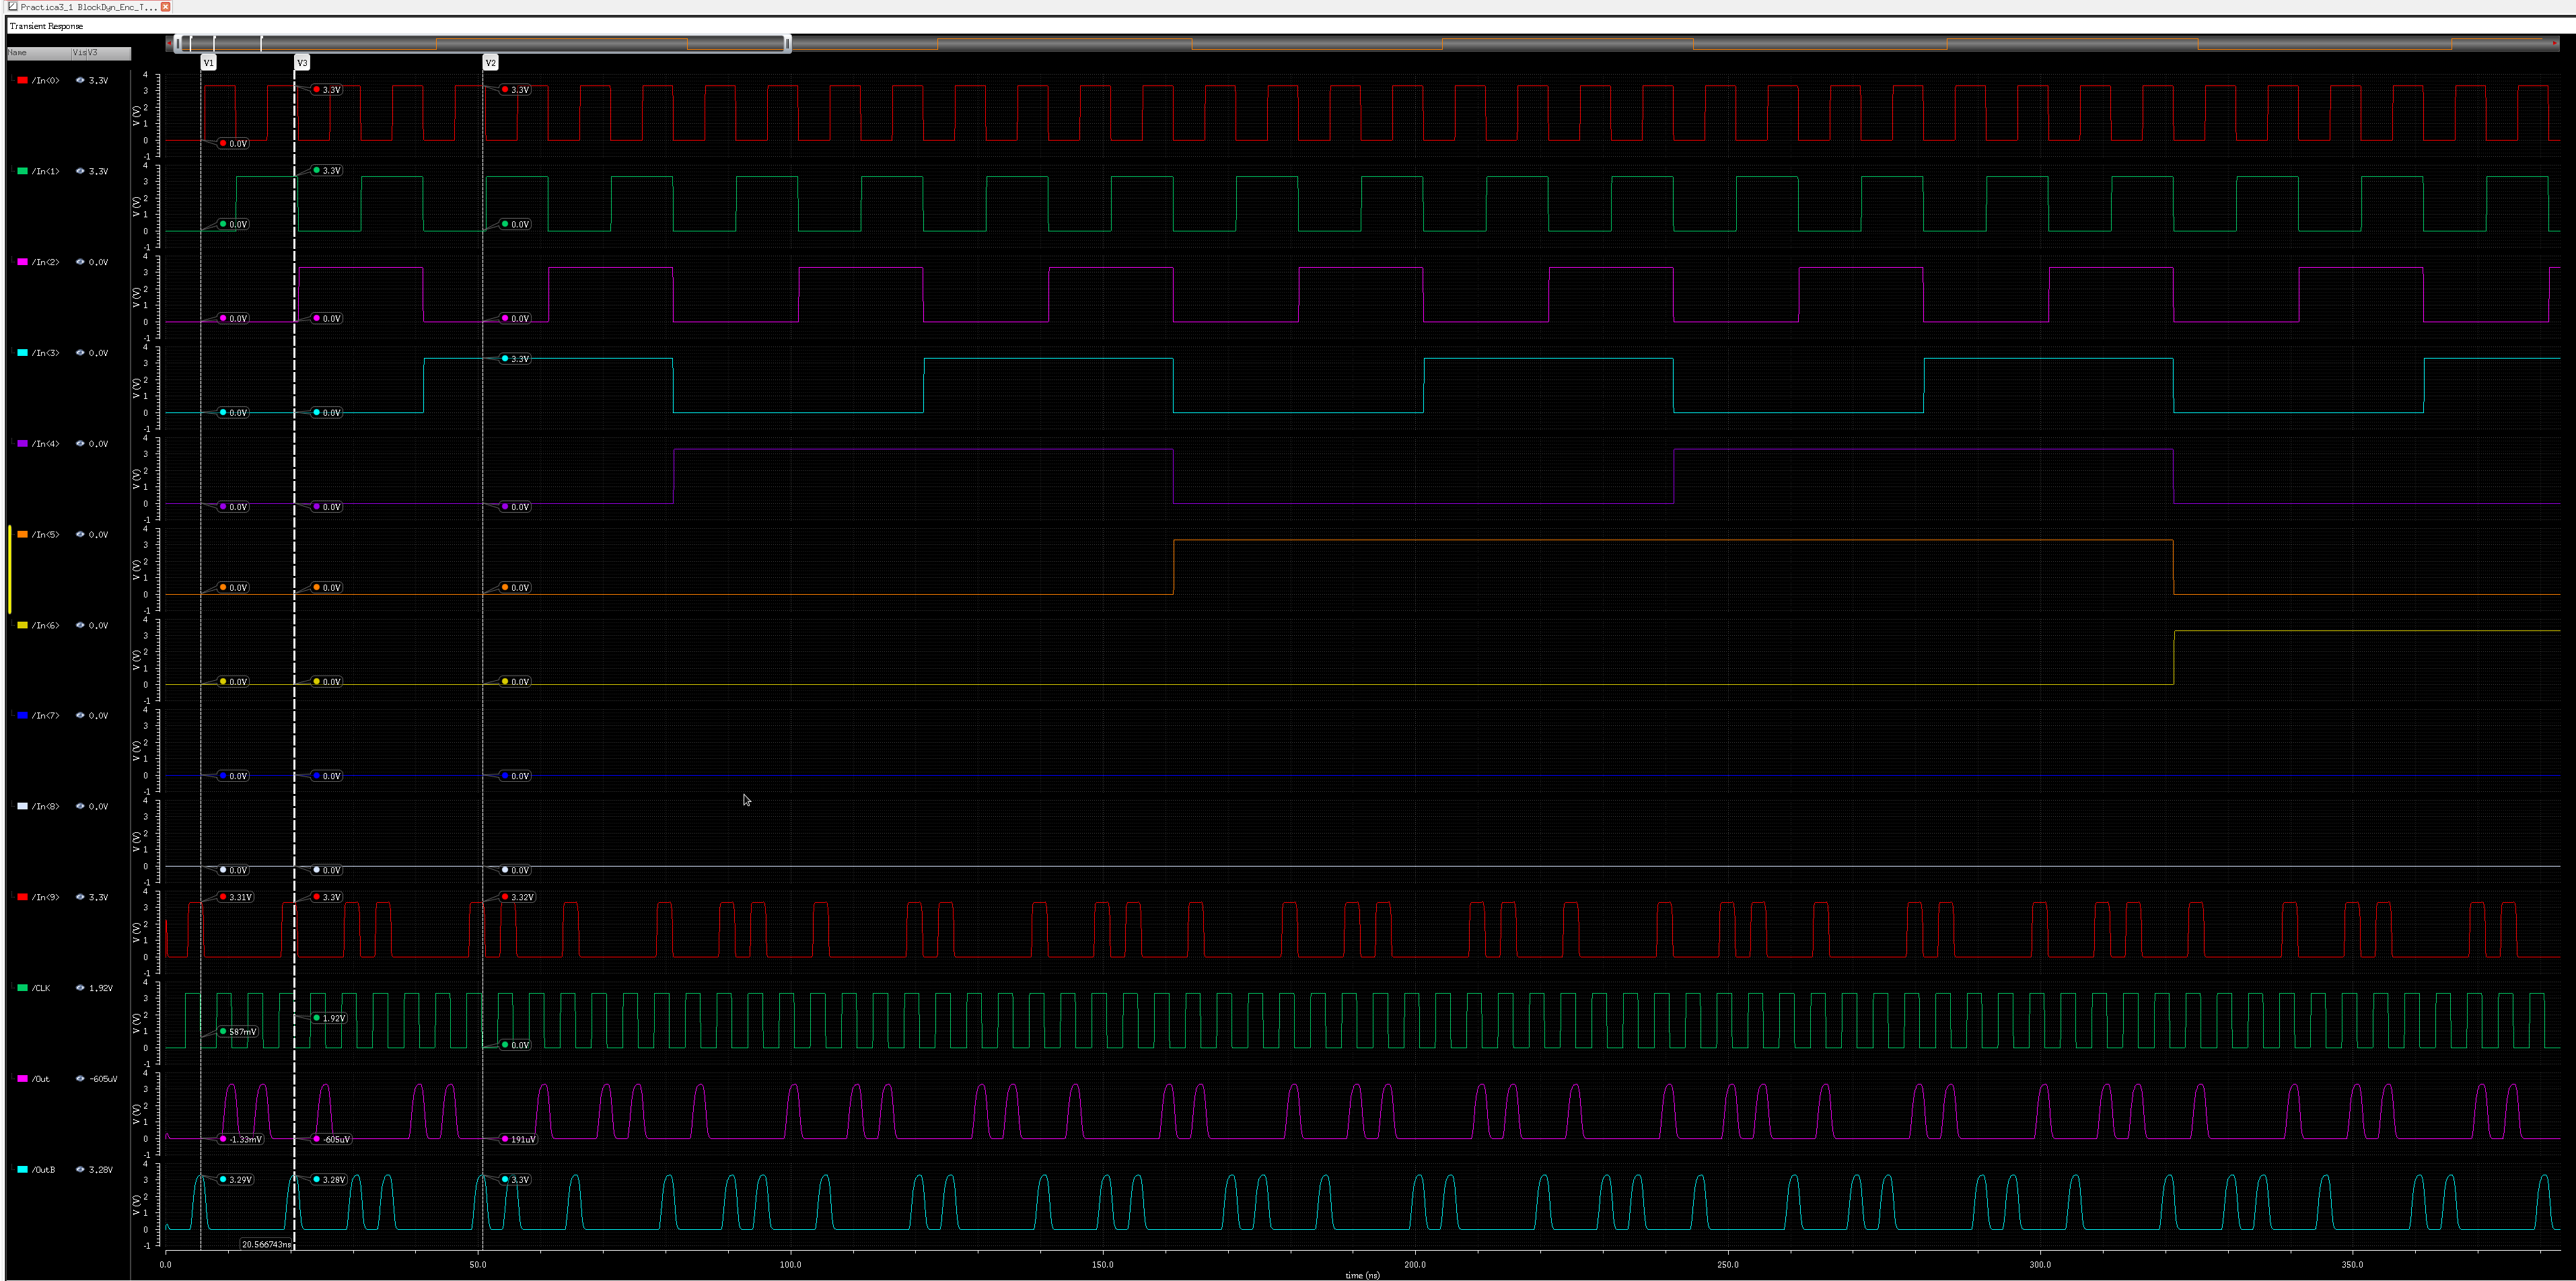
\includegraphics[width=1\textwidth]{figures/GraphEncTB.png}
\caption{Gráfica del banco de pruebas del Encadenado de Etapas Dinámicas}
\label{fig:GraphTBEnc}
\end {center}
\end{figure}
Como se puede observar, la función lógica la hace, de forma correcta, tomando la entrada In<9> como la salida de la primera etapa.  \newpage Tanto la salida Out como su negada OutB son correctas. La forma que presentan (un pulso con un tiempo de subida apreciable) se debe al retardo de propagación que hace que la salida tarde más en alcanzar el nivel alto. La salida de la primera etapa In<9> no presenta este problema ya que obtiene el resultado antes que la segunda etapa, consecuencia de que estemos empleando lógica dominó (las siguientes etapas no se actualizan hasta que no lo han hecho las primeras).

Ahora bien, ¿qué pasaría si encadenáramos mal las etapas y conectáramos la salida de la primera etapa a otra entrada de la segunda? Nos hemos tomado la libertad de simular este caso, cambiando la conexión \say{by name} de la siguiente manera:
\begin{figure}[H]%[!ht]
\begin {center}
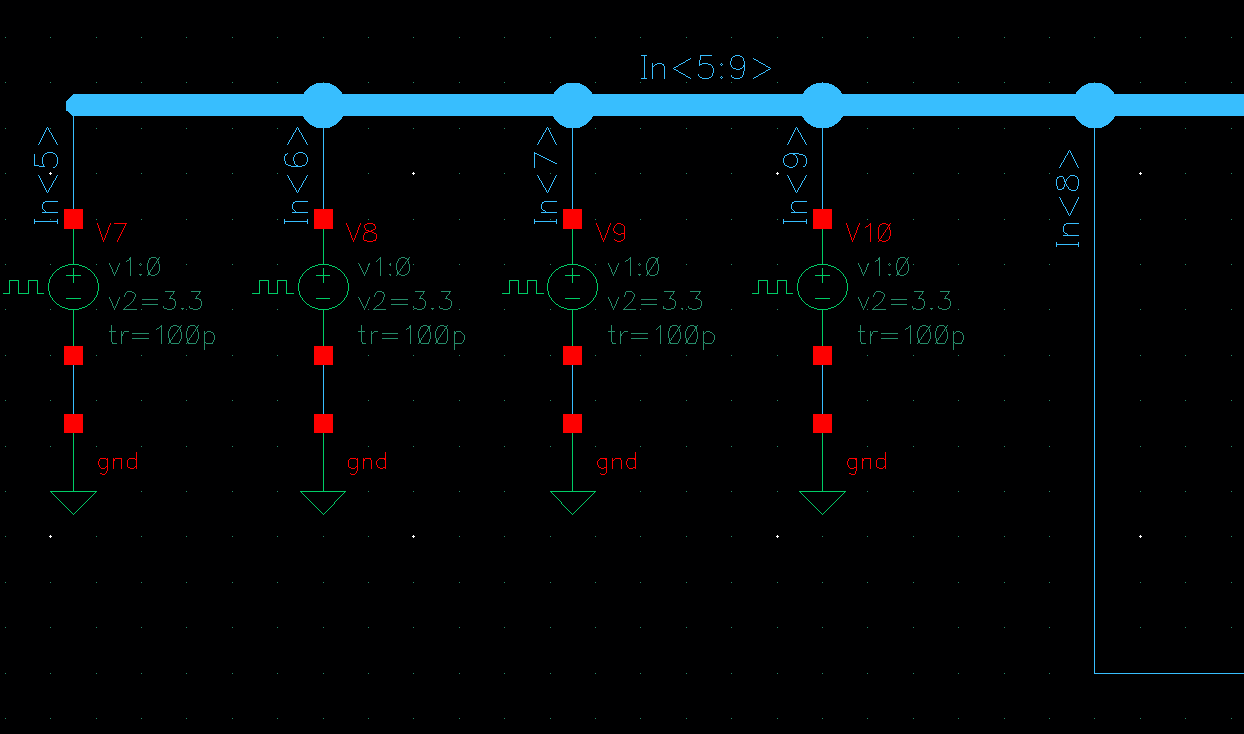
\includegraphics[width=0.75\textwidth]{figures/BlockDynBadSchem.PNG}
\caption{Detalle de la mala conexión de una etapa dinámica con la siguiente}
\label{fig:SchemBadEnc}
\end {center}
\end{figure}
Donde se ha intercambiado la etiqueta In<9> con la etiqueta In<8>. Corriendo una simulación en estas circunstancias, se obtuvo lo siguiente:
\begin{figure}[H]%[!ht]
\hspace{-10mm}
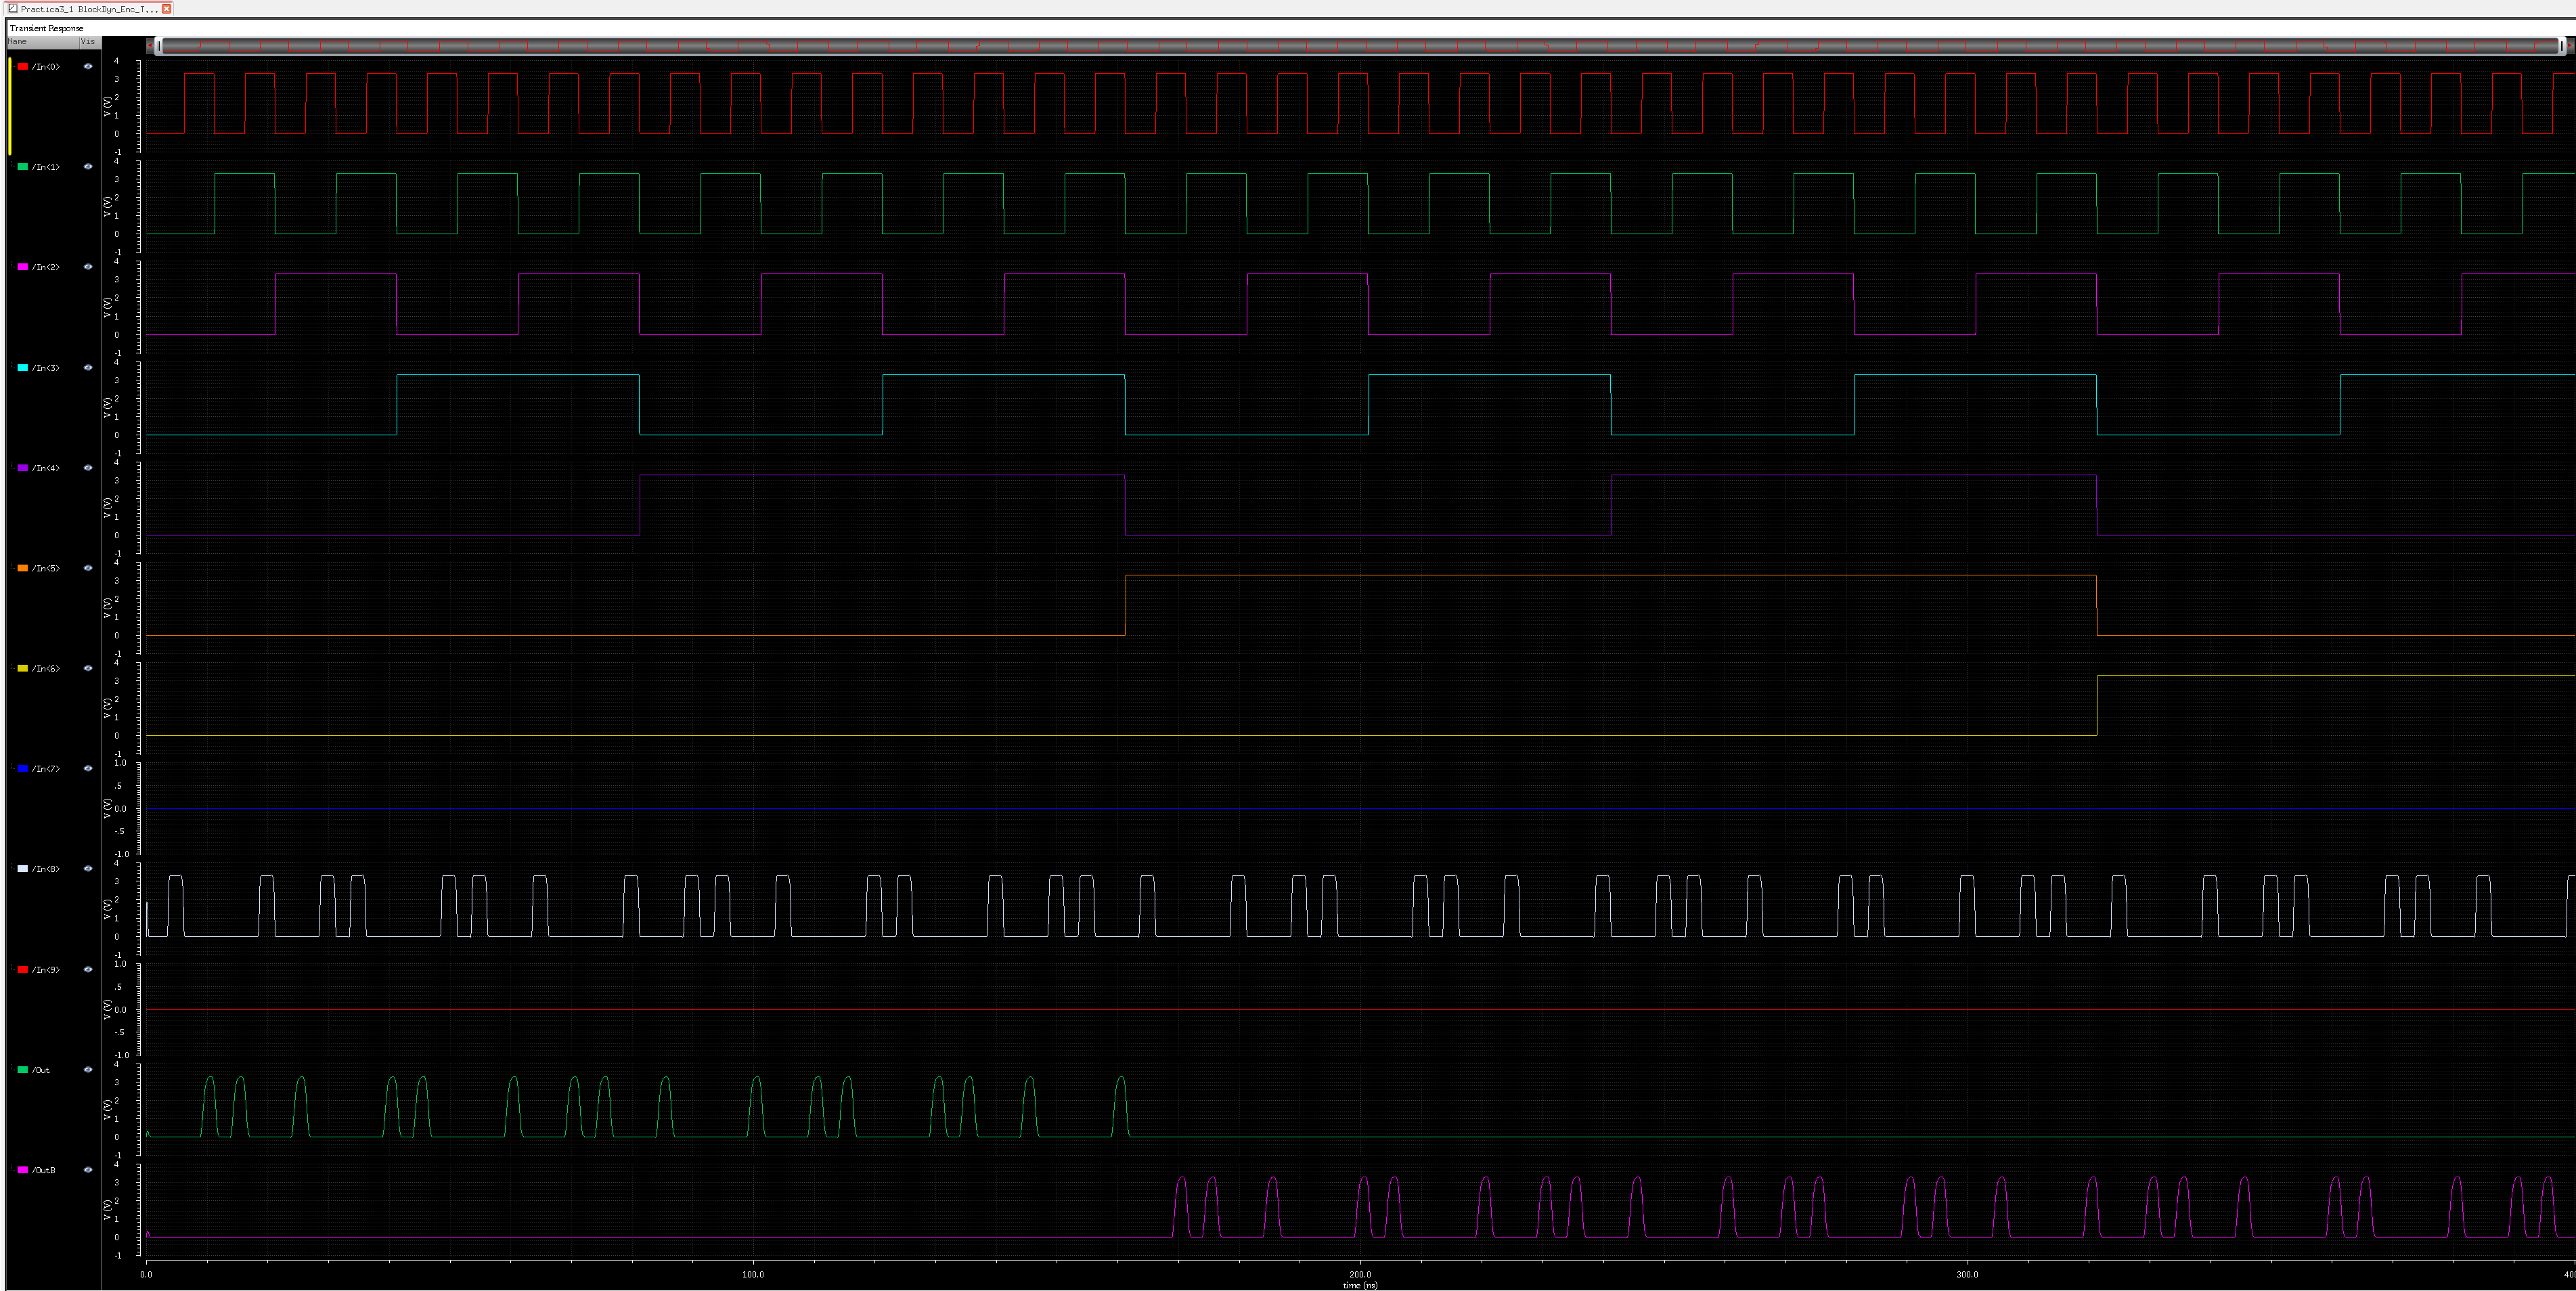
\includegraphics[width=1.2\textwidth]{figures/GraphEncBad.png}
\caption{Simulación de un banco de pruebas con etapas dinámicas incorrectamente encadenadas}
\label{fig:GraphBadEnc}

\end{figure}

Basta con comparar las trazas de Out y OutB para ver que algo no va bien: la salida de OutB no es la negada de Out y, otro comportamiento a tener en cuenta es que sólo una de las dos señales permanece en funcionamiento al mismo tiempo, es decir, en los primeros instantes de la simulación, OutB no muestra signos de ponerse a nivel alto y se queda todo el rato a cero, a pesar de que hay instantes, como se ha visto en la figura \ref{fig:GraphTBEnc}, en los que se debería poner a nivel alto. En conclusión, se hace necesaria la conexión de la forma que se indica en el guion de la práctica. La razón por la que no se podían conectar etapas dinámicas de forma directa era que el retardo de propagación para descargar el primer nodo de salida puede provocar una descarga no deseada de la salida de la siguiente puerta, lo que resulta en una degradación a niveles lógicos. Aquí vemos que hay una degradación que se sigue produciendo en una de las dos salidas.

\restoregeometry


\renewcommand{\baselinestretch}{0.5}
\chapter{Conclusiones}\label{ch:ch4label}
En este apartado, se exponen las justificaciones de los resultados y las conclusiones a las que se han llegado:
\begin{itemize}
    \item \textbf{Lógica CMOS Dinámica:} Se ha comprendido el funcionamiento de la lógica CMOS dinámica así como las ventajas e inconvenientes que esta presenta. Además se ha estudiado el comportamiento eléctrico de un generador de paridad realizado en esta lógica mediante la realización de un esquemático y su posterior simulación. Esto nos ha permitido conocer la función lógica que implementa y diferenciar entre las etapas de precarga y evaluación.
    \item \textbf{Análisis paramétricos:} Yendo más allá en el campo de la simulación, se han corrido sendos análisis paramétricos en frecuencia y en función del ancho de puerta y se han comentado algunos aspectos con respecto al nivel de degradación de la señal y lo que pasaría si el reloj se hace asimétrico llegando, en el caso de la frecuencia a algunos puntos en los que se incumple el $t_{Emin}$ y $t_{Pmax}$.
    \item \textbf{Encadenamiento de etapas dinámicas:} Se ha aprendido la forma correcta de interconectar etapas dinámicas, haciendo hincapié en que es necesaria la lógica dominó para interconectarlas (no vale con interconexión directa) y que se debe hacer de una forma concreta, conectando siempre la salida de la anterior etapa al último bit de la entrada. Si se hace caso omiso de esta regla, el circuito deja de sacar a la salida el resultado esperado tal y como se ha visto en la figura \ref{fig:GraphBadEnc}
\end{itemize}

\printbibliography[heading=bibintoc]
\label{bib:mybiblio}
\end{document}